\documentclass[aspectratio=169,12pt,t]{beamer}

% --- Theme: Metropolis (modern, clean) ---
\usetheme[progressbar=frametitle,numbering=fraction,block=fill]{metropolis}

% --- Fira Sans font (install texlive-fonts-extra if missing) ---
\IfFileExists{FiraSans.sty}{\usepackage[sfdefault]{FiraSans}}{}

% --- Light background with warm accent ---
\definecolor{mDarkTeal}{RGB}{35,55,59}
\definecolor{mLightBrown}{RGB}{235,228,216}
\definecolor{mAccent}{RGB}{140,70,20}

\setbeamercolor{normal text}{fg=mDarkTeal,bg=white}
\setbeamercolor{alerted text}{fg=mAccent}
\setbeamercolor{frametitle}{bg=mDarkTeal,fg=white}
\setbeamercolor{progress bar}{fg=mAccent,bg=mLightBrown}
\setbeamercolor{title separator}{fg=mAccent}
\setbeamercolor{progress bar in head/foot}{fg=mAccent,bg=mLightBrown}
\setbeamercolor{progress bar in section page}{fg=mAccent,bg=mLightBrown}

% --- Packages ---
\usepackage[utf8]{inputenc}
\usepackage{amsmath,amssymb,amsthm}
\usepackage{mathrsfs}
\usepackage{tikz}
\usetikzlibrary{arrows.meta,positioning,calc,decorations.pathreplacing,shapes,patterns}
\usepackage{pgfplots}
\pgfplotsset{compat=1.18}
\usepgfplotslibrary{fillbetween}

% --- TikZ diagram styles (shared across the series) ---
\tikzset{
  axisln/.style={-{Stealth[length=2.6mm]}, line width=0.8pt, gray!75},
  curveln/.style={line width=1.6pt, line cap=round, line join=round},
  projln/.style={dash pattern=on 2.6pt off 2pt, line width=0.7pt},
  guide/.style={-{Stealth[length=2.6mm,width=2.2mm]}, line width=1.1pt},
  box/.style={draw=#1, fill=#1!12, line width=1pt, rounded corners=2pt,
    minimum width=5.6cm, minimum height=1.35cm, align=center, font=\small},
}
% point marker with a white halo: \dotpt{color}{(coord)}
\newcommand{\dotpt}[2]{%
  \fill[white] #2 circle (3.6pt);
  \fill[#1] #2 circle (2.4pt);
}
% open point marker: \opendotpt{color}{(coord)}
\newcommand{\opendotpt}[2]{%
  \fill[white] #2 circle (3.6pt);
  \draw[#1, line width=1pt] #2 circle (2.4pt);
}

% --- Semi-transparent white highlight for text on top of background images ---
\usepackage[most]{tcolorbox}

% Inline highlight: \hl{short text}
\newtcbox{\hl}{%
  nobeforeafter, tcbox raise base,
  colback=white, opacityback=0.6,
  colframe=white, opacityframe=0,
  sharp corners, boxsep=2pt, left=3pt, right=3pt, top=2pt, bottom=2pt%
}

% Block highlight: \begin{hlbox} ... \end{hlbox}  (multi-line, paragraphs, itemize)
% Optional argument accepts any tcolorbox key, e.g. [width=0.6\linewidth]
\newtcolorbox{hlbox}[1][]{%
  enhanced, breakable,
  colback=white, opacityback=0.6,
  colframe=white, opacityframe=0,
  boxsep=3pt, left=6pt, right=6pt, top=4pt, bottom=4pt,
  sharp corners,
  {#1}%
}

% --- Custom colors for content types ---
\definecolor{defcolor}{RGB}{25,85,120}
\definecolor{thmcolor}{RGB}{140,35,35}
\definecolor{proofcolor}{RGB}{35,100,50}
\definecolor{excolor}{RGB}{140,75,10}
\definecolor{remcolor}{RGB}{90,90,90}

% --- Beamer blocks for mathematical content types (semi-transparent) ---
\tcbset{hlblockbase/.style={
  enhanced, breakable,
  coltitle=white, fonttitle=\bfseries,
  opacitybacktitle=0.8, opacityback=0.6,
  opacityframe=0,
  sharp corners,
  boxsep=1pt, left=5pt, right=5pt, top=2pt, bottom=2pt,
  toptitle=1pt, bottomtitle=1pt,
  before upper={\setlength{\abovedisplayskip}{4pt}\setlength{\belowdisplayskip}{4pt}}
}}

\newtcolorbox{defblock}[1]{hlblockbase, title={#1},
  colbacktitle=defcolor, colback=defcolor!15, colframe=defcolor}
\newtcolorbox{thmblock}[1]{hlblockbase, title={#1},
  colbacktitle=thmcolor, colback=thmcolor!15, colframe=thmcolor}
\newtcolorbox{proofblock}[1]{hlblockbase, title={#1},
  colbacktitle=proofcolor, colback=proofcolor!15, colframe=proofcolor}
\newtcolorbox{exblock}[1]{hlblockbase, title={#1},
  colbacktitle=excolor, colback=excolor!15, colframe=excolor}
\newtcolorbox{remblock}[1]{hlblockbase, title={#1},
  colbacktitle=remcolor, colback=remcolor!15, colframe=remcolor}

% --- Metadata ---
\title{Chapter 7: Sequences and Series of Functions}
\subtitle{Section: Uniform Convergence}
\author{Based on Walter Rudin's \emph{Principles of Mathematical Analysis}}
\date{}

\begin{document}

{
\usebackgroundtemplate{%
  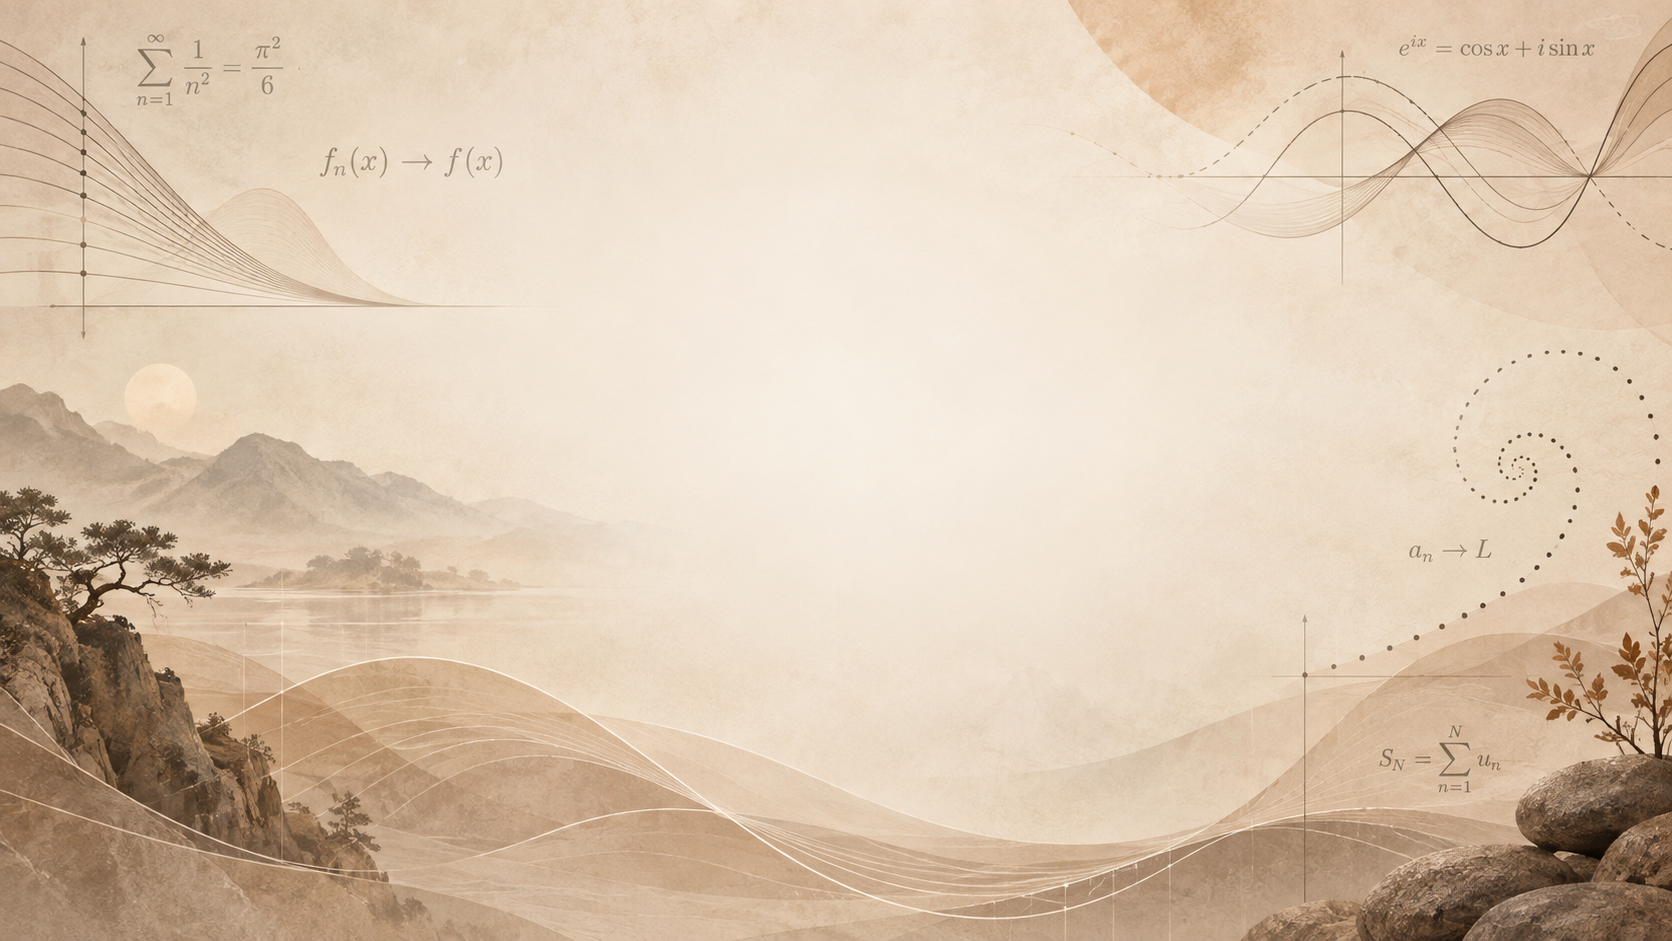
\includegraphics[width=\paperwidth,height=\paperheight,keepaspectratio=false]{chapter_07_bg_00.png}%
}
\begin{frame}[plain]
  \titlepage

  \note{
    Welcome back to Chapter 7, Sequences and Series of Functions. This
    is the second section, Uniform Convergence. In the previous section
    we collected a gallery of examples in which pointwise convergence
    of functions failed to preserve continuity, integrals, and
    derivatives. The common thread was that pointwise convergence lets
    the speed of convergence vary from point to point. In this section
    we introduce the cure: a stronger mode of convergence in which one
    single threshold works for every point at once. We will define
    uniform convergence, prove a Cauchy criterion for it, give a
    practical test in terms of a supremum, and finish with the
    Weierstrass M-test, the workhorse for series of functions. Let's
    begin.
  }
\end{frame}
}

{
\usebackgroundtemplate{%
  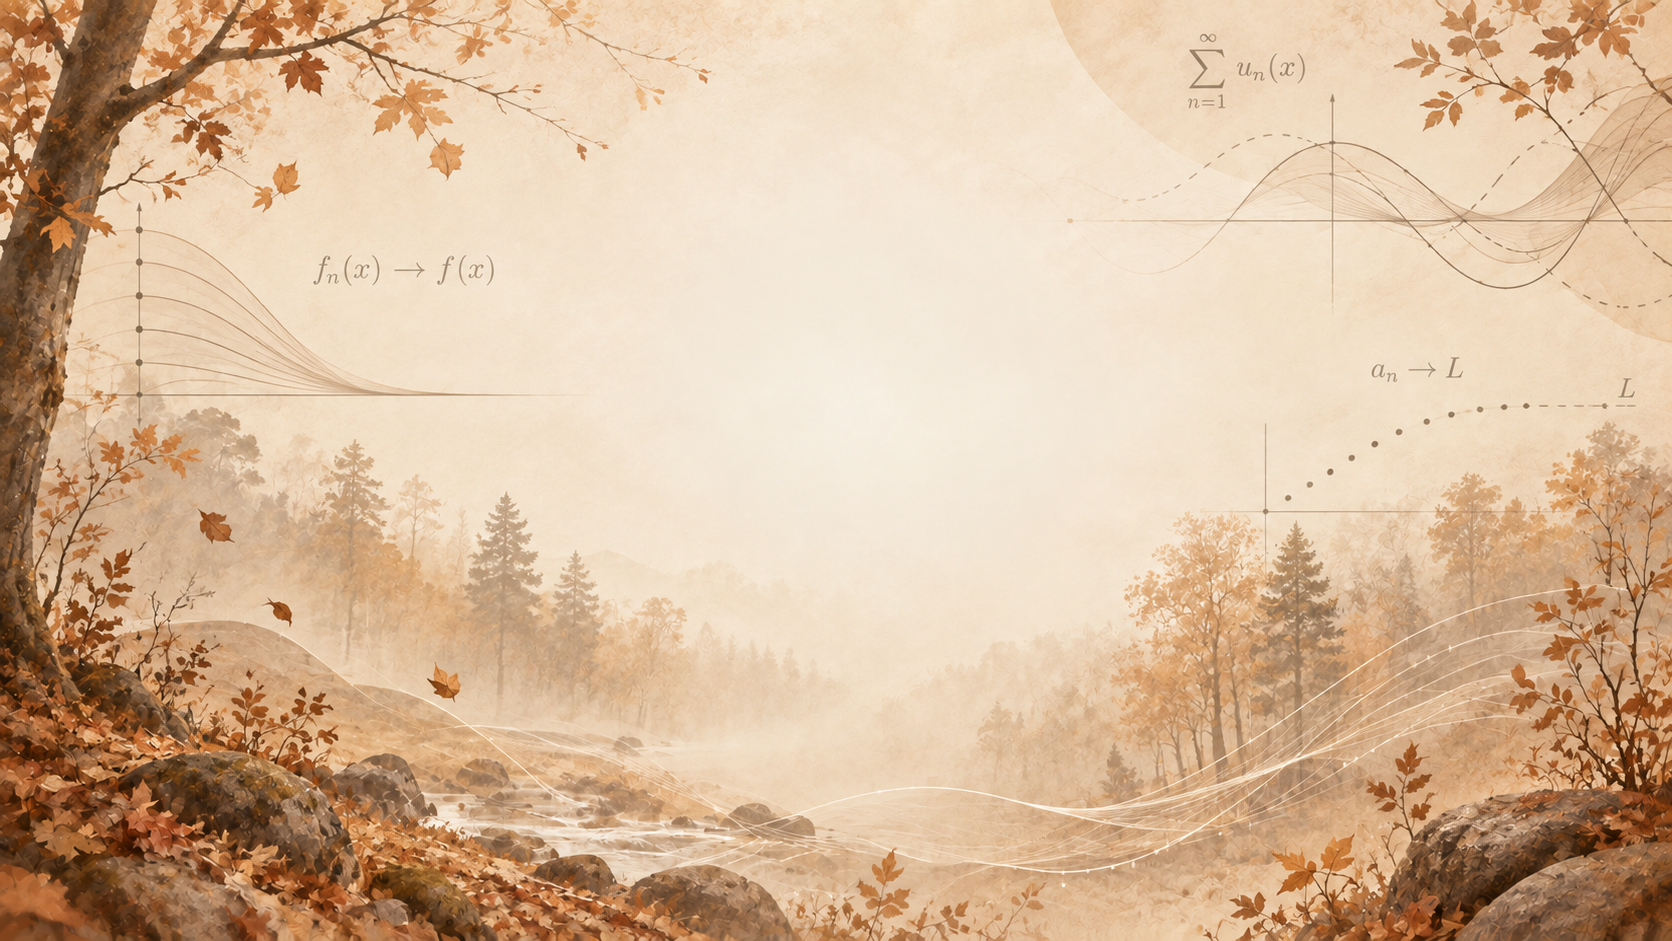
\includegraphics[width=\paperwidth,height=\paperheight,keepaspectratio=false]{chapter_07_bg_01.png}%
}
\begin{frame}[c]{Outline}
  \begin{center}
    \tableofcontents
  \end{center}

  \note{
    Here is the plan. We start with a short motivation that recalls
    where the previous section left off. Then comes Definition 7.7,
    uniform convergence, with a picture of the epsilon tube and a
    careful comparison with pointwise convergence. Next, as a test
    case, we study the powers of "x" on the unit interval, which
    converge pointwise but not uniformly. Then we prove Theorem 7.8,
    the Cauchy criterion for uniform convergence, and state Theorem
    7.9, which reduces uniform convergence to a sequence of suprema;
    we use it to revisit the examples from the previous section.
    Finally, we prove the Weierstrass M-test, Theorem 7.10, apply it
    to a trigonometric series, and see why its converse fails. We close
    with a summary.
  }
\end{frame}

\section{Motivation}

% --- Build 1/3 ---
\begin{frame}{Where We Left Off}
  \begin{hlbox}
  \begin{itemize}
    \item Section 7.1: under \alert{pointwise} convergence $f_n \to f$,
      continuity, integrals, and derivatives can all be \emph{lost}
  \end{itemize}
  \end{hlbox}

  \note{
    Let's recall where we left off. In Section 7.1 we met pointwise
    convergence: "f" sub "n" converges to "f" if, at each point "x",
    the numbers "f" sub "n" of "x" converge to "f" of "x". Then we saw
    five examples showing how weak this is. A series of continuous
    functions had a discontinuous sum. A limit of continuous functions
    was not even integrable. Integrals of "f" sub "n" failed to
    converge to the integral of "f", and derivatives failed to converge
    to the derivative. So what exactly went wrong?
  }
\end{frame}

% --- Build 2/3 ---
\begin{frame}{Where We Left Off}
  \begin{hlbox}
  \begin{itemize}
    \item Section 7.1: under \alert{pointwise} convergence $f_n \to f$,
      continuity, integrals, and derivatives can all be \emph{lost}
    \item The culprit: the threshold $N = N(\varepsilon, x)$ may depend on
      the point $x$, and be \alert{unboundedly large} near a bad point
  \end{itemize}
  \end{hlbox}

  \note{
    The second bullet names the culprit: the order of the quantifiers.
    In pointwise convergence, the point "x" is fixed first, and only then
    do we find a threshold capital "N" beyond which "f" sub "n" of "x" is
    within epsilon of "f" of "x". So capital "N" depends on both epsilon
    and "x". In most of the bad examples there was a region, near the
    origin in Example 7.3, near the rationals in Example 7.4, where the
    required capital "N" grew without bound. The trouble hid exactly
    where convergence was slow.
  }
\end{frame}

% --- Build 3/3 ---
\begin{frame}{Where We Left Off}
  \begin{hlbox}
  \begin{itemize}
    \item Section 7.1: under \alert{pointwise} convergence $f_n \to f$,
      continuity, integrals, and derivatives can all be \emph{lost}
    \item The culprit: the threshold $N = N(\varepsilon, x)$ may depend on
      the point $x$, and be \alert{unboundedly large} near a bad point
    \item The fix: demand \alert{one} $N$ that works for \alert{all} $x \in E$
      simultaneously $\;\Longrightarrow\;$ \emph{uniform convergence}
  \end{itemize}
  \end{hlbox}

  \note{
    The third bullet gives the fix, and it is natural: forbid that
    loophole. We demand that for each epsilon there is one threshold
    capital "N" that works for every point of capital "E" at the same
    time. This is uniform convergence. In the coming sections we will see
    that uniform convergence is enough to preserve continuity and to pass
    limits through integrals, although, as we will also see, derivatives
    need a little more. Before that, here is the roadmap for this
    section.
  }
\end{frame}

\begin{frame}{Roadmap of This Section}
  \vspace{0.6em}
  \begin{center}
  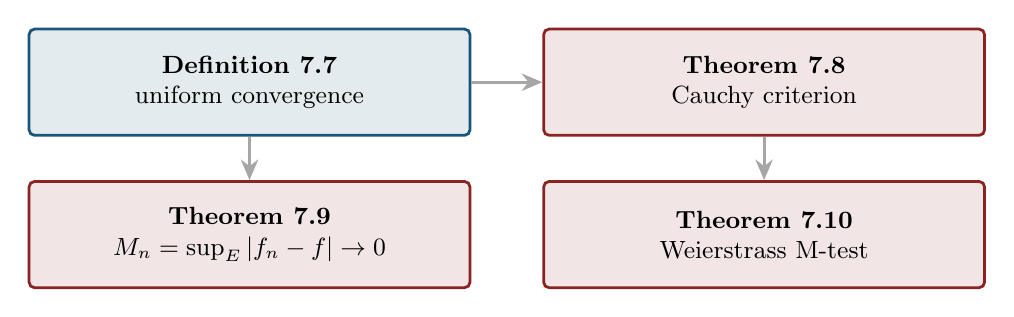
\begin{tikzpicture}[node distance=0.55cm and 0.9cm]
    \node[box=defcolor] (d) {\textbf{Definition 7.7}\\ uniform convergence};
    \node[box=thmcolor, right=of d] (c) {\textbf{Theorem 7.8}\\ Cauchy criterion};
    \node[box=thmcolor, below=of d] (s) {\textbf{Theorem 7.9}\\ $M_n = \sup_E |f_n - f| \to 0$};
    \node[box=thmcolor, below=of c] (w) {\textbf{Theorem 7.10}\\ Weierstrass M-test};
    \draw[guide, gray!70] (d) -- (c);
    \draw[guide, gray!70] (d) -- (s);
    \draw[guide, gray!70] (c) -- (w);
  \end{tikzpicture}
  \end{center}

  \vspace{0.5em}
  \hl{\textbf{Goal:} practical tools to \alert{verify} uniform convergence.}

  \note{
    The diagram shows the four results of this section and how they
    depend on each other. The blue box at the top left is Definition
    7.7, uniform convergence itself. From it, gray arrows lead to two
    red theorem boxes. To the right, Theorem 7.8, the Cauchy criterion,
    which characterizes uniform convergence without knowing the limit
    function. Below, Theorem 7.9, which says uniform convergence
    means that the largest distance between "f" sub "n" and "f" tends
    to zero. Finally, the Cauchy criterion feeds into Theorem 7.10, the
    Weierstrass M-test, which is the most convenient test for series
    of functions. The goal is to have practical tools for verifying
    uniform convergence. Let's start with the definition.
  }
\end{frame}
}

{
\usebackgroundtemplate{%
  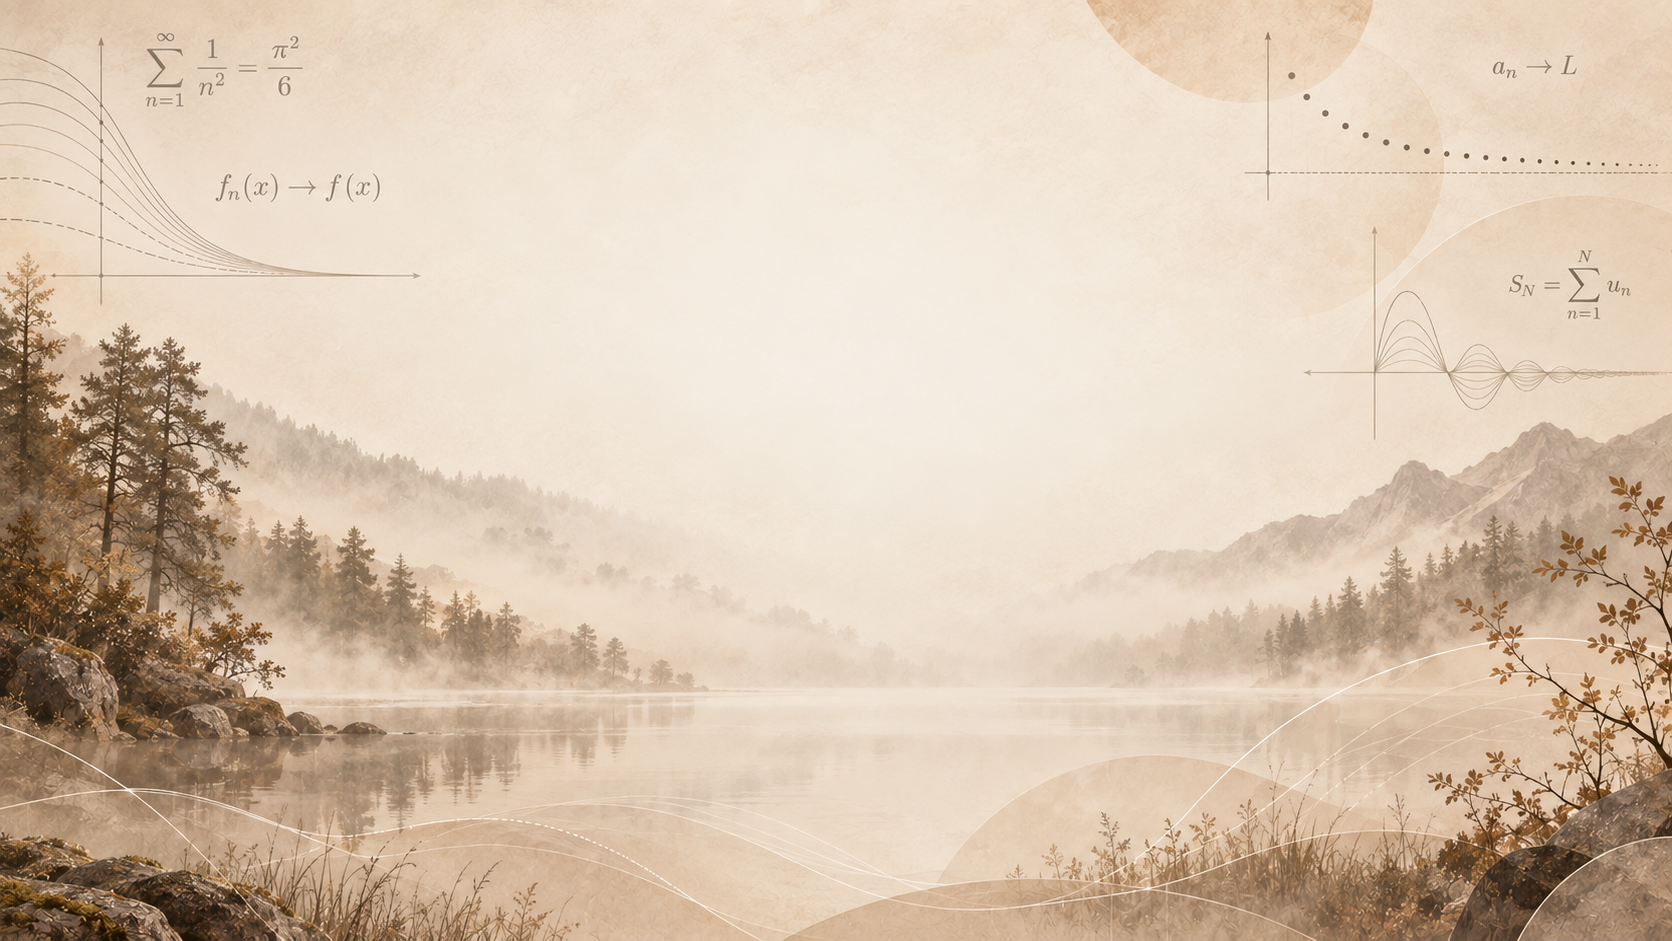
\includegraphics[width=\paperwidth,height=\paperheight,keepaspectratio=false]{chapter_07_bg_02.png}%
}
\section{Uniform Convergence}

\begin{frame}{Definition 7.7: Uniform Convergence}
  \begin{defblock}{Definition 7.7}
    A sequence of functions $\{f_n\}$, $n = 1, 2, 3, \dots$, \alert{converges
    uniformly} on $E$ to a function $f$ if for every $\varepsilon > 0$ there is an
    integer $N$ such that $n \geq N$ implies
    \begin{equation}
      |f_n(x) - f(x)| \leq \varepsilon \tag{12}
    \end{equation}
    for \alert{all} $x \in E$.
  \end{defblock}

  \vspace{0.3em}
  \hl{\textbf{Key point:} $N$ depends on $\varepsilon$ \emph{only}, not on $x$.}

  \note{
    Here is Definition 7.7. The sequence "f" sub "n" converges uniformly
    on capital "E" to "f" if for every epsilon there is an integer
    capital "N" such that, from index capital "N" on, inequality 12 holds
    at every point "x" of capital "E" at once. A helpful way to read it:
    think of epsilon as an error tolerance. Uniform convergence promises
    a single stage capital "N" after which "f" sub "n" approximates "f"
    within that tolerance everywhere, so one approximation is good
    enough for the whole set. With pointwise convergence, the stage you
    need depends on where you look. That is what the line below the box
    stresses: capital "N" depends on epsilon only. Let's see what this
    means geometrically.
  }
\end{frame}

\begin{frame}[c]{Uniform Convergence: The $\varepsilon$-Tube}
  \begin{center}
  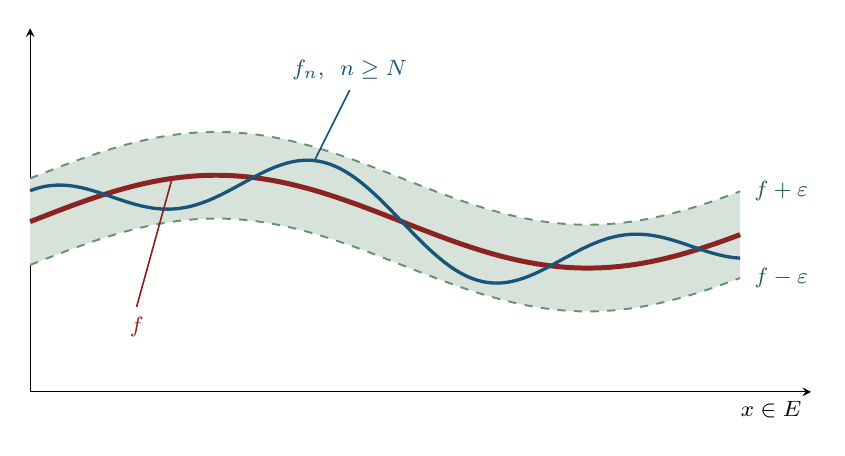
\begin{tikzpicture}
    \begin{axis}[
      width=11.5cm, height=6.2cm,
      axis lines=left,
      xmin=0, xmax=3.3, ymin=0, ymax=2.35,
      xtick=\empty, ytick=\empty,
      xlabel={$x \in E$}, xlabel style={font=\footnotesize, at={(1,0)}, anchor=north east},
      legend style={font=\scriptsize, at={(0.99,0.99)}, anchor=north east,
        draw=none, fill=white, fill opacity=0.8, text opacity=1},
      clip=false,
    ]
      \addplot[name path=upper, proofcolor!70, line width=0.7pt, dashed, domain=0:3, samples=120]
        {1.1 + 0.3*sin(deg(2*x)) + 0.28};
      \addplot[name path=lower, proofcolor!70, line width=0.7pt, dashed, domain=0:3, samples=120]
        {1.1 + 0.3*sin(deg(2*x)) - 0.28};
      \addplot[proofcolor!18] fill between[of=upper and lower];
      \addplot[thmcolor, line width=1.8pt, domain=0:3, samples=120]
        {1.1 + 0.3*sin(deg(2*x))};
      \addplot[defcolor, line width=1.2pt, domain=0:3, samples=200]
        {1.1 + 0.3*sin(deg(2*x)) + 0.2*cos(deg(5*x))};
      \node[proofcolor, font=\footnotesize, anchor=west] at (axis cs:3.02,1.296) {$f + \varepsilon$};
      \node[proofcolor, font=\footnotesize, anchor=west] at (axis cs:3.02,0.736) {$f - \varepsilon$};
      \draw[thmcolor, line width=0.6pt] (axis cs:0.6,1.38) -- (axis cs:0.45,0.55)
        node[below, font=\footnotesize] {$f$};
      \draw[defcolor, line width=0.6pt] (axis cs:1.2,1.49) -- (axis cs:1.35,1.95)
        node[above, font=\footnotesize] {$f_n$, \ $n \geq N$};
    \end{axis}
  \end{tikzpicture}
  \end{center}

  \note{
    Here is the picture to keep in mind. The horizontal axis represents
    the set capital "E". The thick red curve is the limit function "f";
    its label sits below the tube on the left, joined to the curve by a
    thin red line. Around it, the green shaded region between the two
    dashed green curves, "f" plus epsilon above and "f" minus epsilon
    below, is a tube reaching a distance epsilon above and below "f".
    Uniform convergence says: however thin the tube, there is a threshold
    capital "N" such that every "f" sub "n" with "n" at least capital "N"
    lies entirely inside it, over the whole set. The blue wiggly curve,
    labeled at the top with a thin blue line, is one such "f" sub "n": it
    wanders around "f", but never leaves the green region. Pointwise
    convergence would only require that, above each individual point,
    the values eventually enter the tube, possibly at wildly different
    times. Next, let's compare the two definitions side by side.
  }
\end{frame}

% --- Build 1/2 ---
\begin{frame}{Pointwise vs.\ Uniform: Order of Quantifiers}
  \begin{remblock}{Pointwise on $E$}
    $\alert{\forall x \in E}\;\; \forall \varepsilon > 0\;\; \exists N\;\;
      \forall n \geq N: \quad |f_n(x) - f(x)| \leq \varepsilon$
  \end{remblock}
  \begin{defblock}{Uniform on $E$}
    $\forall \varepsilon > 0\;\; \exists N\;\; \alert{\forall x \in E}\;\;
      \forall n \geq N: \quad |f_n(x) - f(x)| \leq \varepsilon$
  \end{defblock}

  \vspace{0.3em}
  \hl{Pointwise: $N = N(\varepsilon, x)$. \qquad Uniform: $N = N(\varepsilon)$.}

  \note{
    The two boxes contain the same ingredients; only the phrase for all
    "x" in capital "E", highlighted in orange, has moved. Think of a
    game. An opponent names a tolerance epsilon, and you answer with a
    threshold capital "N". In the gray pointwise box, the opponent must
    reveal the point "x" first, so you can tailor capital "N" to it. In
    the blue uniform box, you commit to capital "N" first, and only then
    may the opponent test you at any point "x". That is the summary in
    the line below the boxes.
  }
\end{frame}

% --- Build 2/2 ---
\begin{frame}{Pointwise vs.\ Uniform: Order of Quantifiers}
  \begin{remblock}{Pointwise on $E$}
    $\alert{\forall x \in E}\;\; \forall \varepsilon > 0\;\; \exists N\;\;
      \forall n \geq N: \quad |f_n(x) - f(x)| \leq \varepsilon$
  \end{remblock}
  \begin{defblock}{Uniform on $E$}
    $\forall \varepsilon > 0\;\; \exists N\;\; \alert{\forall x \in E}\;\;
      \forall n \geq N: \quad |f_n(x) - f(x)| \leq \varepsilon$
  \end{defblock}

  \vspace{0.3em}
  \hl{Pointwise: $N = N(\varepsilon, x)$. \qquad Uniform: $N = N(\varepsilon)$.}

  \vspace{0.3em}
  \begin{hlbox}
  \begin{itemize}
    \item Uniform $\;\Longrightarrow\;$ pointwise \ (same $N$ for every $x$)
    \item Pointwise $\;\not\Longrightarrow\;$ uniform \ (example coming up)
  \end{itemize}
  \end{hlbox}

  \note{
    Two consequences follow. First, as Rudin remarks, every uniformly
    convergent sequence is pointwise convergent: if one capital "N"
    works for all points, then in particular it works for each point.
    Second, the converse is false. Pointwise convergence only
    guarantees a threshold for each point separately, and these
    thresholds may be unbounded as the point moves around. We will see
    a concrete example of this in a moment. But first, the definition
    for series.
  }
\end{frame}

\begin{frame}{Uniform Convergence of Series}
  \begin{defblock}{Definition 7.7 (series)}
    The series $\sum f_n(x)$ \alert{converges uniformly} on $E$ if the sequence
    $\{s_n\}$ of partial sums
    \[
      s_n(x) = \sum_{i=1}^{n} f_i(x)
    \]
    converges uniformly on $E$.
  \end{defblock}

  \vspace{0.3em}
  \hl{\textbf{As always:} a series of functions \emph{is} the sequence of its
  partial sums.}

  \note{
    For series, nothing new is needed. We form the partial sums "s" sub
    "n", the sum of the first "n" functions, and each partial sum is
    again a function on capital "E". The series converges uniformly if
    this sequence of partial sum functions converges uniformly. This
    matters because many important functions, such as power series and
    trigonometric series, are defined as sums of series. One useful
    remark for later: the difference of two partial sums, "s" sub "m"
    minus the partial sum with index "n" minus 1, is just the block of
    terms from "n" to "m". This is how the Cauchy criterion will enter
    the M-test. Now, the promised example.
  }
\end{frame}
}

{
\usebackgroundtemplate{%
  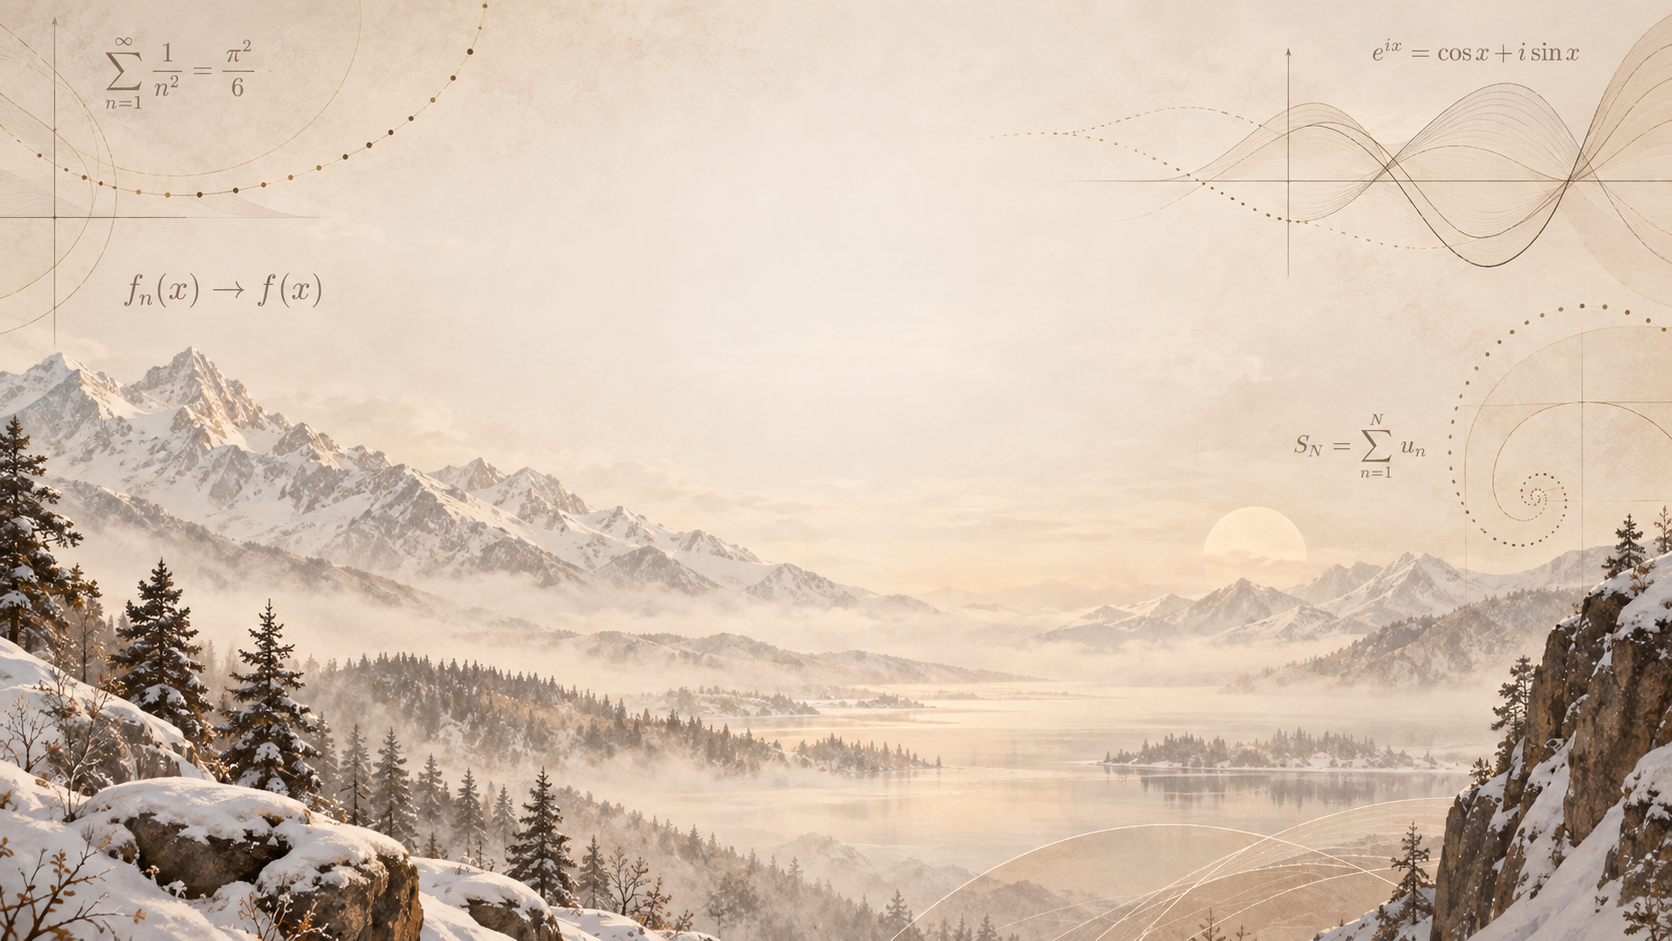
\includegraphics[width=\paperwidth,height=\paperheight,keepaspectratio=false]{chapter_07_bg_03.png}%
}
\section{A Test Case: $x^n$ on $[0,1]$}

% --- Build 1/3 ---
\begin{frame}{Test Case: $f_n(x) = x^n$}
  \begin{exblock}{Pointwise limit on $[0, 1]$}
    \[
      f_n(x) = x^n \;\longrightarrow\; f(x) =
      \begin{cases} 0, & 0 \leq x < 1,\\ 1, & x = 1. \end{cases}
    \]
  \end{exblock}

  \note{
    Let's test the definitions on the simplest interesting example, "x"
    to the "n" on the closed unit interval. For "x" strictly between 0
    and 1 the powers tend to zero, at 0 they are all zero, and at 1 they
    are all equal to 1. So the pointwise limit "f", shown in the box, is
    zero on the half open interval and 1 at the right endpoint. Every "f"
    sub "n" is continuous but the limit is not, so by the next section
    the convergence cannot be uniform. Let's see this directly.
  }
\end{frame}

% --- Build 2/3 ---
\begin{frame}{Test Case: $f_n(x) = x^n$}
  \begin{exblock}{Pointwise limit on $[0, 1]$}
    \[
      f_n(x) = x^n \;\longrightarrow\; f(x) =
      \begin{cases} 0, & 0 \leq x < 1,\\ 1, & x = 1. \end{cases}
    \]
  \end{exblock}

  \begin{hlbox}
  \begin{itemize}
    \item For $0 < x < 1$, $0 < \varepsilon < 1$: \ $x^n \leq \varepsilon \iff n \geq
      \dfrac{\log \varepsilon}{\log x} = N(\varepsilon, x) \;\xrightarrow[x \to 1^-]{}\; \alert{\infty}$
  \end{itemize}
  \end{hlbox}

  \note{
    Fix epsilon between 0 and 1, and a point "x" between 0 and 1. Then
    "x" to the "n" is at most epsilon exactly when "n" is at least the
    logarithm of epsilon divided by the logarithm of "x". Both
    logarithms are negative, so this ratio is positive. It is the
    smallest threshold that works at the point "x". But as "x" moves
    toward 1, the logarithm of "x" tends to zero, and the threshold
    blows up to infinity. Points close to 1 need ever larger
    thresholds, so no single capital "N" works on the whole interval.
  }
\end{frame}

% --- Build 3/3 ---
\begin{frame}{Test Case: $f_n(x) = x^n$}
  \begin{exblock}{Pointwise limit on $[0, 1]$}
    \[
      f_n(x) = x^n \;\longrightarrow\; f(x) =
      \begin{cases} 0, & 0 \leq x < 1,\\ 1, & x = 1. \end{cases}
    \]
  \end{exblock}

  \begin{hlbox}
  \begin{itemize}
    \item For $0 < x < 1$, $0 < \varepsilon < 1$: \ $x^n \leq \varepsilon \iff n \geq
      \dfrac{\log \varepsilon}{\log x} = N(\varepsilon, x) \;\xrightarrow[x \to 1^-]{}\; \alert{\infty}$
    \item \alert{Not uniform} on $[0, 1]$: \ $\sup_{0 \leq x < 1} |x^n - f(x)| = 1$ for every $n$
    \item \alert{Uniform} on $[0, a]$, $a < 1$: \ $x^n \leq a^n \to 0$ for all $x \in [0, a]$
  \end{itemize}
  \end{hlbox}

  \note{
    The last two bullets make this precise. For "x" below 1 the error is
    just "x" to the "n", and its supremum is 1 for every "n", because "x"
    can be taken as close to 1 as we like. So for epsilon less than 1, no
    "f" sub "n" lies within epsilon of "f" on the whole interval: not
    uniform. But if we stay away from 1, on the interval from 0 to "a"
    with "a" less than 1, every "x" to the "n" is at most "a" to the
    "n", which tends to zero. One threshold works everywhere there: the
    convergence is uniform. Here is the picture.
  }
\end{frame}

\begin{frame}[c]{Test Case: Every $x^n$ Escapes the Tube Near $1$}
  \begin{center}
  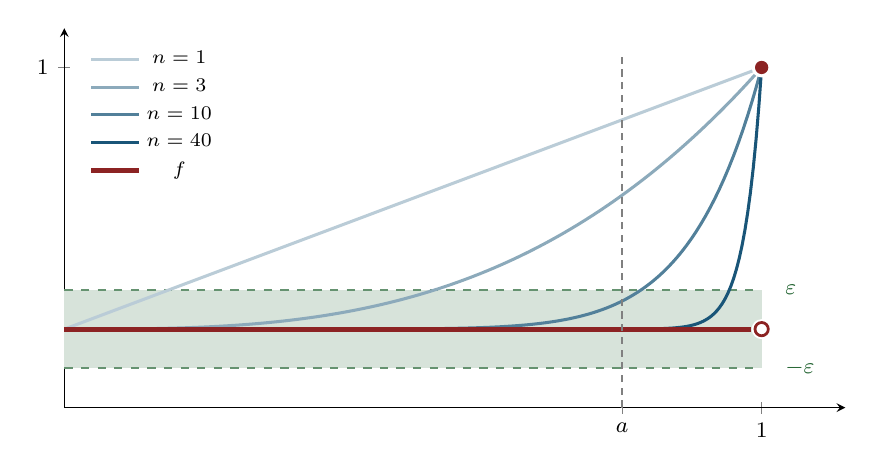
\begin{tikzpicture}
    \begin{axis}[
      width=11.5cm, height=6.4cm,
      axis lines=left,
      xmin=0, xmax=1.12, ymin=-0.3, ymax=1.15,
      xtick={0.8,1}, xticklabels={$a$,$1$},
      ytick={1},
      tick label style={font=\footnotesize},
      legend style={font=\scriptsize, at={(0.02,0.97)}, anchor=north west,
        draw=none, fill=white, fill opacity=0.8, text opacity=1},
      clip=false,
    ]
      \fill[proofcolor!18] (axis cs:0,-0.15) rectangle (axis cs:1,0.15);
      \draw[proofcolor!70, dashed, line width=0.7pt] (axis cs:0,0.15) -- (axis cs:1,0.15);
      \draw[proofcolor!70, dashed, line width=0.7pt] (axis cs:0,-0.15) -- (axis cs:1,-0.15);
      \addplot[defcolor!30, line width=1.1pt, domain=0:1, samples=100] {x};
      \addlegendentry{$n = 1$}
      \addplot[defcolor!50, line width=1.1pt, domain=0:1, samples=100] {x^3};
      \addlegendentry{$n = 3$}
      \addplot[defcolor!75, line width=1.1pt, domain=0:1, samples=150] {x^10};
      \addlegendentry{$n = 10$}
      \addplot[defcolor, line width=1.1pt, domain=0:1, samples=250] {x^40};
      \addlegendentry{$n = 40$}
      \addplot[thmcolor, line width=1.8pt, domain=0:0.985, samples=2] {0};
      \addlegendentry{$f$}
      \opendotpt{thmcolor}{(axis cs:1,0)}
      \dotpt{thmcolor}{(axis cs:1,1)}
      \draw[projln, gray] (axis cs:0.8,-0.3) -- (axis cs:0.8,1.05);
      \node[proofcolor, font=\footnotesize, anchor=west] at (axis cs:1.02,0.15) {$\varepsilon$};
      \node[proofcolor, font=\footnotesize, anchor=west] at (axis cs:1.02,-0.15) {$-\varepsilon$};
    \end{axis}
  \end{tikzpicture}
  \end{center}

  \note{
    The blue curves are "x" to the "n" for "n" equal to 1, 3, 10, and
    40, in increasingly dark blue. The thick red segment along the axis
    is the limit "f", which is zero on the half open interval, with an
    open red circle at "x" equals 1 on the axis and a filled red dot at
    height 1, the value "f" of 1. The green strip between the dashed
    lines labeled epsilon and minus epsilon is the epsilon tube around
    "f". Every blue curve starts inside the strip, but has to climb to
    height 1 at "x" equals 1, so near 1 it always escapes the tube. That
    is the failure of uniform convergence. Now look to the left of the
    dashed gray vertical line at "x" equals "a". There the curves for
    "n" equal to 10 and 40 already lie inside the strip, while the
    curves for 1 and 3 do not yet: on the interval from 0 to "a", one
    threshold works everywhere. Next, a criterion that does not require
    knowing the limit.
  }
\end{frame}
}

{
\usebackgroundtemplate{%
  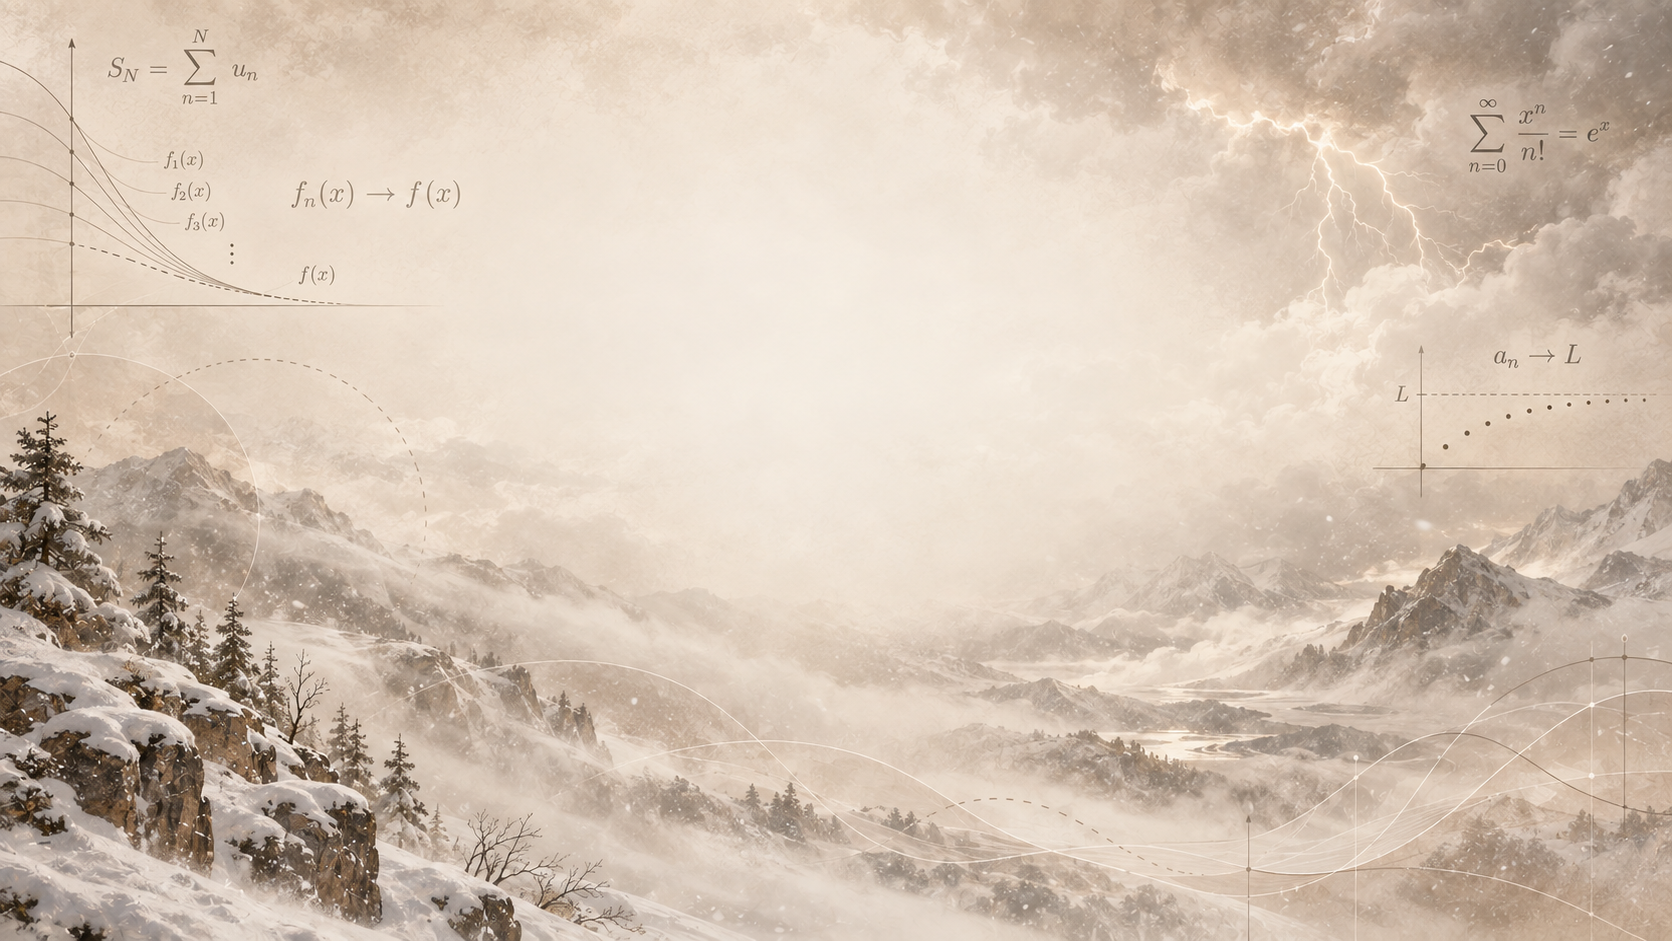
\includegraphics[width=\paperwidth,height=\paperheight,keepaspectratio=false]{chapter_07_bg_04.png}%
}
\section{The Cauchy Criterion}

% --- Build 1/2 ---
\begin{frame}{Theorem 7.8: Cauchy Criterion for Uniform Convergence}
  \begin{thmblock}{Theorem 7.8}
    The sequence of functions $\{f_n\}$, defined on $E$, converges uniformly on
    $E$ \alert{if and only if} for every $\varepsilon > 0$ there exists an integer
    $N$ such that $m \geq N$, $n \geq N$, $x \in E$ implies
    \begin{equation}
      |f_n(x) - f_m(x)| \leq \varepsilon. \tag{13}
    \end{equation}
  \end{thmblock}

  \note{
    Here is Theorem 7.8, the Cauchy criterion for uniform convergence.
    Recall that a sequence of numbers is a Cauchy sequence if its terms
    eventually stay within epsilon of each other, and that in the real
    line such sequences converge. The theorem says the same thing for
    functions, with one extra demand: in inequality 13, the index
    capital "N" must work for all points "x" of capital "E" at once.
    Geometrically, from stage capital "N" onward, the graphs of any two
    functions "f" sub "n" and "f" sub "m" lie within epsilon of each
    other everywhere; the whole tail of the sequence bunches together
    uniformly.
  }
\end{frame}

% --- Build 2/2 ---
\begin{frame}{Theorem 7.8: Cauchy Criterion for Uniform Convergence}
  \begin{thmblock}{Theorem 7.8}
    The sequence of functions $\{f_n\}$, defined on $E$, converges uniformly on
    $E$ \alert{if and only if} for every $\varepsilon > 0$ there exists an integer
    $N$ such that $m \geq N$, $n \geq N$, $x \in E$ implies
    \begin{equation}
      |f_n(x) - f_m(x)| \leq \varepsilon. \tag{13}
    \end{equation}
  \end{thmblock}

  \vspace{0.3em}
  \begin{hlbox}
  \textbf{Why it is useful:} condition (13) mentions only the $f_n$,
  \alert{not the limit $f$}.\\
  We can prove uniform convergence \emph{before} we know what $f$ is.
  \end{hlbox}

  \note{
    Why is this useful? Look at condition 13: it only involves the
    functions "f" sub "n" themselves, and never mentions the limit
    function "f". Very often, especially for series of functions, we
    have no closed formula for the limit. The Cauchy criterion lets us
    prove uniform convergence anyway, and the limit function comes out
    as a byproduct. This is exactly how we will prove the Weierstrass
    M-test at the end of this section. Let's see the proof strategy.
  }
\end{frame}

\begin{frame}{Proof Strategy: Theorem 7.8}
  \begin{hlbox}
  \textbf{Two directions:}
  \vspace{0.3em}
  \begin{enumerate}
    \item[($\Rightarrow$)] Uniform $\Rightarrow$ Cauchy: insert $f$ and use
      \alert{triangle inequality} with $\varepsilon/2$.
    \item[($\Leftarrow$)] Cauchy $\Rightarrow$ uniform:
      \begin{enumerate}
        \item[(a)] each $\{f_n(x)\}$ is a Cauchy sequence of numbers, so it
          converges (Theorem 3.11); call the limit $f(x)$;
        \item[(b)] let $m \to \infty$ in (13) to get a bound
          \alert{uniform in $x$}.
      \end{enumerate}
  \end{enumerate}
  \end{hlbox}

  \note{
    The proof has two directions. For the forward direction, from
    uniform convergence to the Cauchy condition, we insert the limit
    function between "f" sub "n" and "f" sub "m" and use the triangle
    inequality, with epsilon over 2 on each side. The converse has two
    parts. Part "a": at each fixed point "x", condition 13 says that
    the numbers "f" sub "n" of "x" form a Cauchy sequence, so by
    Theorem 3.11 they converge; this defines the candidate limit "f".
    Part "b": we let "m" tend to infinity in inequality 13 and get a
    bound on the distance to "f" that is the same for all "x". Let's
    do the first direction.
  }
\end{frame}

\begin{frame}{Proof of Theorem 7.8 --- ($\Rightarrow$) Uniform Implies Cauchy}
  \begin{proofblock}{Step 1: Uniform $\Rightarrow$ Cauchy}
    Let $f_n \to f$ uniformly on $E$. Choose $N$ such that $n \geq N$, $x \in E$
    implies
    \[
      |f_n(x) - f(x)| \leq \frac{\varepsilon}{2}.
    \]
    Then for $n \geq N$, $m \geq N$, $x \in E$:
    \[
      |f_n(x) - f_m(x)| \leq |f_n(x) - f(x)| + |f(x) - f_m(x)|
      \leq \frac{\varepsilon}{2} + \frac{\varepsilon}{2} = \boxed{\varepsilon}.
    \]
  \end{proofblock}

  \note{
    Suppose "f" sub "n" converges uniformly to "f" on capital "E". We
    apply the definition with epsilon over 2 instead of epsilon: there
    is a capital "N" such that for every "n" at least capital "N" and
    every "x" in capital "E", "f" sub "n" of "x" is within epsilon over
    2 of "f" of "x". Now take two indices "n" and "m", both at least
    capital "N". The triangle inequality, with "f" of "x" inserted in
    the middle, bounds the distance between "f" sub "n" of "x" and "f"
    sub "m" of "x" by the sum of two terms, each at most epsilon over
    2. The total is at most epsilon. Since the same capital "N" served
    every "x", condition 13 holds uniformly. That is the easy
    direction.
  }
\end{frame}

% --- Build 1/2 ---
\begin{frame}{Proof of Theorem 7.8 --- ($\Leftarrow$) Cauchy Implies Uniform}
  \begin{proofblock}{Step 2: The pointwise limit exists}
    Assume the Cauchy condition (13). For each fixed $x \in E$, $\{f_n(x)\}$ is a
    \alert{Cauchy sequence} of numbers, so by Theorem 3.11 it converges. Put
    \[
      f(x) = \lim_{n \to \infty} f_n(x) \qquad (x \in E).
    \]
    Thus $f_n \to f$ pointwise. \emph{Still to show: uniformly.}
  \end{proofblock}

  \note{
    Now the converse. Assume the Cauchy condition 13 holds. Freeze a
    point "x" in capital "E". Then condition 13 says in particular that
    the sequence of numbers "f" sub "n" of "x" is a Cauchy sequence.
    Recall Theorem 3.11: in the real line, and more generally in any
    Euclidean space, every Cauchy sequence converges. So the limit
    exists, and we call it "f" of "x". Doing this at every point
    defines a function "f" on capital "E", and "f" sub "n" converges to
    "f" pointwise. But pointwise is not enough; we still have to show
    the convergence is uniform.
  }
\end{frame}

% --- Build 2/2 ---
\begin{frame}{Proof of Theorem 7.8 --- ($\Leftarrow$) Cauchy Implies Uniform}
  \begin{proofblock}{Step 2: The pointwise limit exists}
    Assume the Cauchy condition (13). For each fixed $x \in E$, $\{f_n(x)\}$ is a
    \alert{Cauchy sequence} of numbers, so by Theorem 3.11 it converges. Put
    \[
      f(x) = \lim_{n \to \infty} f_n(x) \qquad (x \in E).
    \]
    Thus $f_n \to f$ pointwise. \emph{Still to show: uniformly.}
  \end{proofblock}
  \begin{proofblock}{Step 3: Let $m \to \infty$ in (13)}
    Given $\varepsilon > 0$, take $N$ from (13). Fix $n \geq N$ and $x \in E$;
    since $f_m(x) \to f(x)$ as $m \to \infty$,
    \begin{equation}
      \boxed{|f_n(x) - f(x)| \leq \varepsilon} \qquad (n \geq N,\; x \in E). \tag{14}
    \end{equation}
  \end{proofblock}

  \note{
    Here is the key step. Given epsilon, take the capital "N" from
    condition 13, and fix any "n" at least capital "N" and any point
    "x". For every "m" at least capital "N", "f" sub "n" of "x" and "f"
    sub "m" of "x" are within epsilon. Now let "m" go to infinity while
    "n" and "x" stay fixed. Since "f" sub "m" of "x" converges to "f" of
    "x", and an inequality of the form less than or equal to survives the limit, we get
    inequality 14. Crucially, capital "N" was chosen before "x", so it
    works for every "x" at once. That is uniform convergence.
  }
\end{frame}
}

{
\usebackgroundtemplate{%
  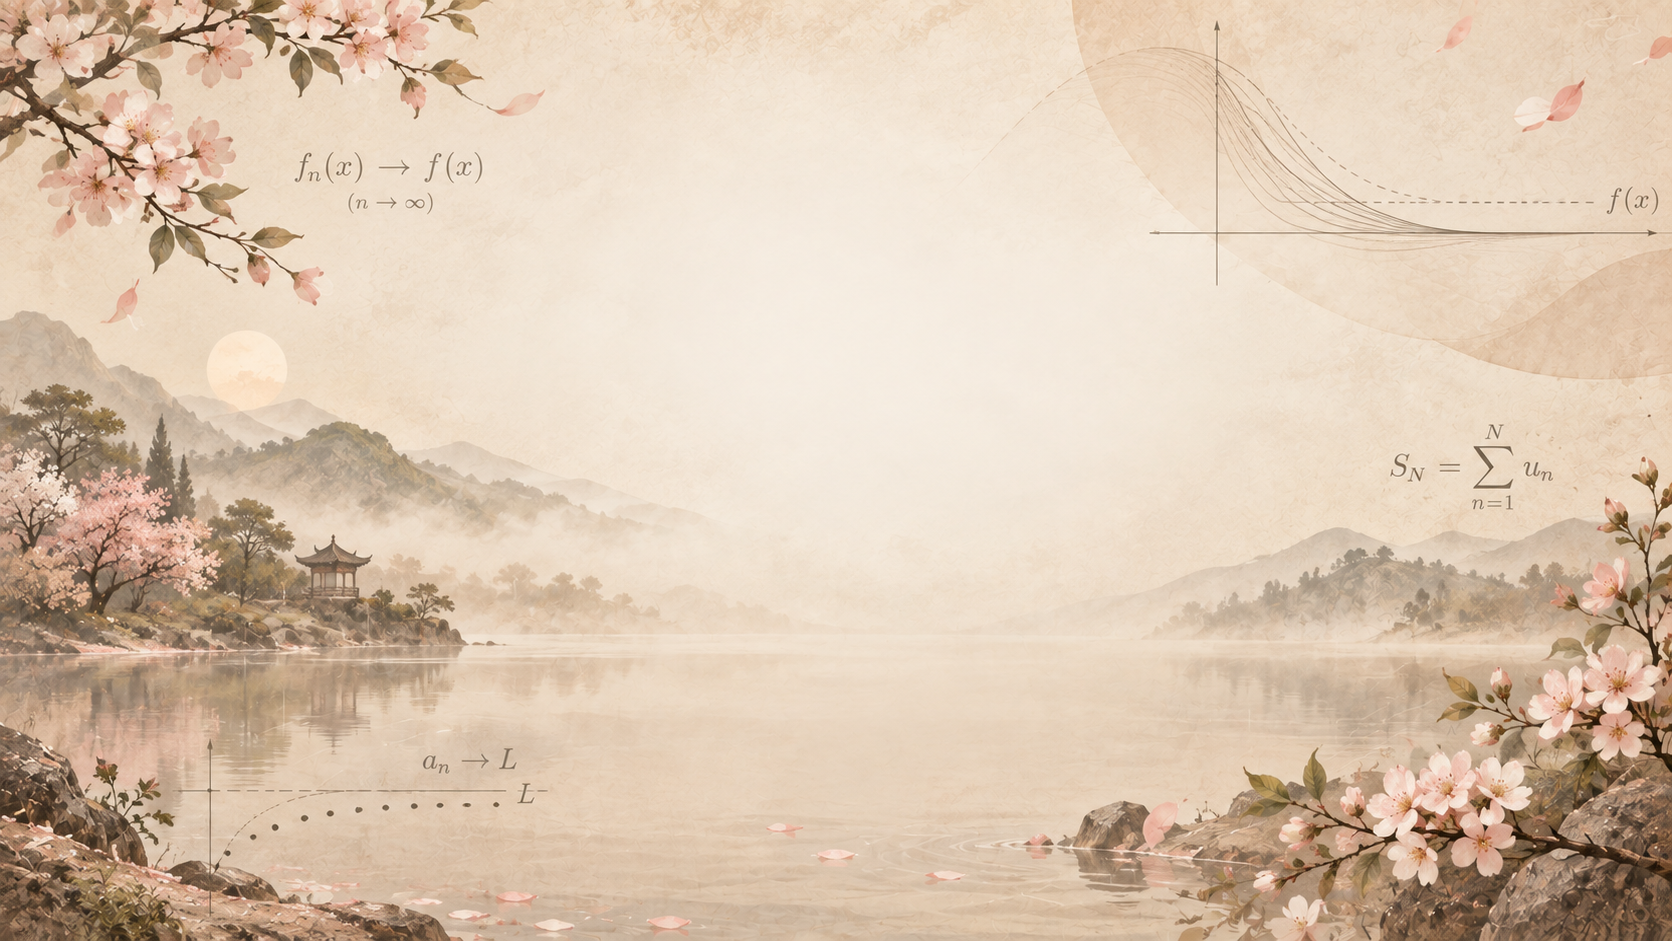
\includegraphics[width=\paperwidth,height=\paperheight,keepaspectratio=false]{chapter_07_bg_05.png}%
}
\section{The Supremum Criterion}

% --- Build 1/2 ---
\begin{frame}{Theorem 7.9: Uniform Convergence via Suprema}
  \begin{thmblock}{Theorem 7.9}
    Suppose $\displaystyle\lim_{n \to \infty} f_n(x) = f(x)$ \ $(x \in E)$. Put
    \[
      M_n = \sup_{x \in E} |f_n(x) - f(x)|.
    \]
    Then $f_n \to f$ \alert{uniformly} on $E$ if and only if
    $\alert{M_n \to 0}$ as $n \to \infty$.
  \end{thmblock}

  \note{
    Rudin calls the next criterion sometimes useful; in practice we
    reach for it constantly. Suppose "f" sub "n" converges to
    "f" pointwise, so we know the candidate limit. Let capital "M" sub
    "n" be the supremum over capital "E" of the distance between "f" sub
    "n" of "x" and "f" of "x": the worst case error at stage "n".
    Theorem 7.9 says the convergence is uniform exactly when these worst
    case errors tend to zero. Functions are reduced to one sequence of
    numbers.
  }
\end{frame}

% --- Build 2/2 ---
\begin{frame}{Theorem 7.9: Uniform Convergence via Suprema}
  \begin{thmblock}{Theorem 7.9}
    Suppose $\displaystyle\lim_{n \to \infty} f_n(x) = f(x)$ \ $(x \in E)$. Put
    \[
      M_n = \sup_{x \in E} |f_n(x) - f(x)|.
    \]
    Then $f_n \to f$ \alert{uniformly} on $E$ if and only if
    $\alert{M_n \to 0}$ as $n \to \infty$.
  \end{thmblock}
  \begin{proofblock}{Proof (immediate from Definition 7.7)}
    $|f_n(x) - f(x)| \leq \varepsilon$ for \emph{all} $x \in E$
    $\iff$ $M_n \leq \varepsilon$ \\
    (a sup is $\leq \varepsilon$ iff every value is).
  \end{proofblock}

  \note{
    Rudin omits the proof as an immediate consequence of Definition
    7.7, and the green box shows why. Saying the distance is at most
    epsilon for all "x" in capital "E" means epsilon is an upper bound
    for these distances, which is the same as saying their least upper
    bound, capital "M" sub "n", is at most epsilon. So uniform
    convergence reads: for every epsilon there is a capital "N" with
    capital "M" sub "n" at most epsilon whenever "n" is at least
    capital "N". That is exactly the statement that capital "M" sub
    "n" tends to zero. Let's picture it.
  }
\end{frame}

\begin{frame}[c]{Theorem 7.9: $M_n$ Is the Largest Vertical Gap}
  \begin{center}
  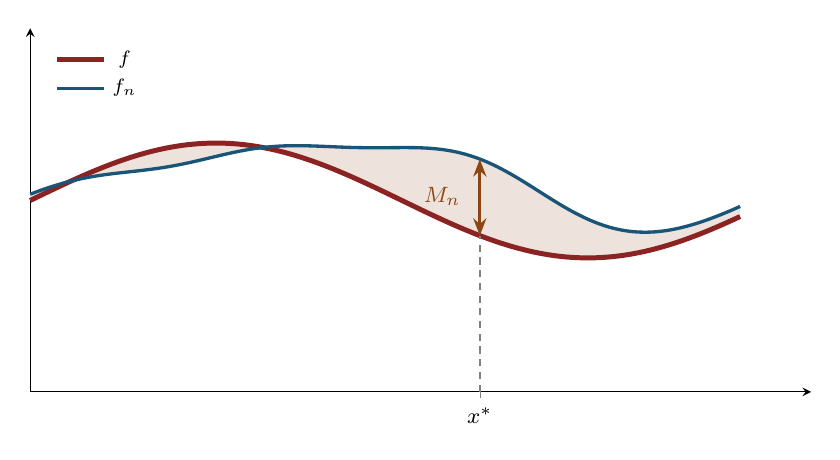
\begin{tikzpicture}
    \begin{axis}[
      width=11.5cm, height=6.2cm,
      axis lines=left,
      xmin=0, xmax=3.3, ymin=0, ymax=1.9,
      xtick={1.9}, xticklabels={$x^*$}, ytick=\empty,
      tick label style={font=\footnotesize},
      legend style={font=\scriptsize, at={(0.02,0.97)}, anchor=north west,
        draw=none, fill=white, fill opacity=0.8, text opacity=1},
      clip=false,
    ]
      \addplot[name path=fcurve, thmcolor, line width=1.8pt, domain=0:3, samples=150]
        {1 + 0.3*sin(deg(2*x))};
      \addlegendentry{$f$}
      \addplot[name path=fncurve, defcolor, line width=1.2pt, domain=0:3, samples=200]
        {1 + 0.3*sin(deg(2*x)) + 0.05 + 0.35*exp(-4*(x-1.9)^2) - 0.15*exp(-6*(x-0.6)^2)};
      \addlegendentry{$f_n$}
      \addplot[mAccent!15] fill between[of=fcurve and fncurve];
      \draw[projln, gray] (axis cs:1.9,0) -- (axis cs:1.9,0.816);
      \draw[{Stealth[length=2.2mm]}-{Stealth[length=2.2mm]}, mAccent, line width=1.1pt]
        (axis cs:1.9,0.816) -- (axis cs:1.9,1.216);
      \node[mAccent, font=\footnotesize, anchor=east] at (axis cs:1.86,1.02) {$M_n$};
    \end{axis}
  \end{tikzpicture}
  \end{center}

  \note{
    In the picture, the thick red curve is the limit "f" and the blue
    curve is one approximating function "f" sub "n". The light orange
    shading fills the region between them; its height above each point
    is the error at that point. On the left, the blue curve dips slightly
    below the red one, and the error there counts in absolute value. The
    orange double arrow, labeled capital "M" sub "n" on its left, sits at
    the point "x" star where the vertical gap is largest; its length is
    capital "M" sub "n". Pointwise convergence says the gap above each
    fixed point shrinks to zero. Uniform convergence says more: the
    largest gap, wherever it occurs, shrinks to zero. If the worst point
    keeps producing a gap of fixed size, possibly by moving around as
    "n" grows, the convergence is not uniform. Let's revisit the
    examples with this tool.
  }
\end{frame}

% --- Build 1/4 ---
\begin{frame}{Revisiting the Examples with $M_n$}
  \renewcommand{\arraystretch}{1.35}
  \begin{hlbox}
  \begin{center}
  \begin{tabular}{l l l l}
    \textbf{Sequence} & \textbf{Limit} & $\boldsymbol{M_n}$ & \textbf{Uniform?} \\ \hline
    $x^n$ on $[0,1)$ & $0$ & $1$ & \alert{no} \\
  \end{tabular}
  \end{center}
  \end{hlbox}

  \note{
    The table collects examples we already know. For each one we compute
    the worst case error capital "M" sub "n" and read off the verdict.
    The first row is our test case, "x" to the "n" on the half open
    interval from 0 to 1. The limit is zero, so capital "M" sub "n" is
    simply the supremum of "x" to the "n", which equals 1 for every "n".
    It does not tend to zero, so by Theorem 7.9 the convergence is not
    uniform, confirming the picture we just saw. Next, Example 7.3.
  }
\end{frame}

% --- Build 2/4 ---
\begin{frame}{Revisiting the Examples with $M_n$}
  \renewcommand{\arraystretch}{1.35}
  \begin{hlbox}
  \begin{center}
  \begin{tabular}{l l l l}
    \textbf{Sequence} & \textbf{Limit} & $\boldsymbol{M_n}$ & \textbf{Uniform?} \\ \hline
    $x^n$ on $[0,1)$ & $0$ & $1$ & \alert{no} \\
    Ex.\ 7.3: $s_n = \sum_{k=0}^{n} \frac{x^2}{(1+x^2)^k}$ on $\mathbb{R}$
      & $f$ & $\sup_{x \neq 0} (1+x^2)^{-n} = 1$ & \alert{no} \\
  \end{tabular}
  \end{center}
  \end{hlbox}

  \note{
    Second row: Example 7.3, the series whose terms are "x" squared
    divided by the quantity 1 plus "x" squared, raised to the power "k".
    Its partial sums "s" sub "n" converge to the function "f" that equals
    1 plus "x" squared away from the origin and 0 at the origin. Summing
    the geometric series, the error at a point "x" other than 0 turns out
    to be 1 divided by the quantity 1 plus "x" squared, raised to the
    power "n". As "x" approaches 0 this error approaches 1, so the
    supremum is 1 for every "n". Not uniform, which is consistent with
    the discontinuous sum.
  }
\end{frame}

% --- Build 3/4 ---
\begin{frame}{Revisiting the Examples with $M_n$}
  \renewcommand{\arraystretch}{1.35}
  \begin{hlbox}
  \begin{center}
  \begin{tabular}{l l l l}
    \textbf{Sequence} & \textbf{Limit} & $\boldsymbol{M_n}$ & \textbf{Uniform?} \\ \hline
    $x^n$ on $[0,1)$ & $0$ & $1$ & \alert{no} \\
    Ex.\ 7.3: $s_n = \sum_{k=0}^{n} \frac{x^2}{(1+x^2)^k}$ on $\mathbb{R}$
      & $f$ & $\sup_{x \neq 0} (1+x^2)^{-n} = 1$ & \alert{no} \\
    Ex.\ 7.6: $n^2 x (1 - x^2)^n$ on $[0,1]$ & $0$ & $\to \infty$ & \alert{no} \\
  \end{tabular}
  \end{center}
  \end{hlbox}

  \note{
    Third row: Example 7.6, the escaping bumps. Here "f" sub "n" of "x"
    is "n" squared times "x" times the quantity 1 minus "x" squared,
    raised to the power "n", on the unit interval. The limit is zero at
    every point. But the bump peaks near "x" equals 1 over the square
    root of 2 "n", and its height there grows like "n" to the power three
    halves. So capital "M" sub "n", the height of the bump, tends to
    infinity. Far from tending to zero, the worst case error explodes.
    Not uniform, and indeed the integrals failed to converge to the
    integral of the limit.
  }
\end{frame}

% --- Build 4/4 ---
\begin{frame}{Revisiting the Examples with $M_n$}
  \renewcommand{\arraystretch}{1.35}
  \begin{hlbox}
  \begin{center}
  \begin{tabular}{l l l l}
    \textbf{Sequence} & \textbf{Limit} & $\boldsymbol{M_n}$ & \textbf{Uniform?} \\ \hline
    $x^n$ on $[0,1)$ & $0$ & $1$ & \alert{no} \\
    Ex.\ 7.3: $s_n = \sum_{k=0}^{n} \frac{x^2}{(1+x^2)^k}$ on $\mathbb{R}$
      & $f$ & $\sup_{x \neq 0} (1+x^2)^{-n} = 1$ & \alert{no} \\
    Ex.\ 7.6: $n^2 x (1 - x^2)^n$ on $[0,1]$ & $0$ & $\to \infty$ & \alert{no} \\
    Ex.\ 7.5: $\frac{\sin nx}{\sqrt{n}}$ on $\mathbb{R}$ & $0$ & $\frac{1}{\sqrt{n}} \to 0$
      & \textcolor{proofcolor}{\textbf{yes}} \\
  \end{tabular}
  \end{center}
  \end{hlbox}

  \vspace{0.4em}
  \begin{hlbox}
  \textbf{But:} in Ex.\ 7.5, $f_n'(0) = \sqrt{n} \to \infty$. Uniform convergence
  alone does \alert{not} control derivatives.
  \end{hlbox}

  \note{
    The last row is a surprise. Example 7.5 was sine of "n" "x" over the
    square root of "n", on the whole real line. Since the sine is at
    most 1 in size, capital "M" sub "n" is 1 over the square root of
    "n", which tends to zero: this convergence is uniform. And yet, as
    the line below the table recalls, the derivative at 0 equals the
    square root of "n", which blows up, while the limit has derivative
    zero. Uniform convergence will rescue continuity and integrals, but
    derivatives need an extra hypothesis. Now, a test tailored to series.
  }
\end{frame}
}

{
\usebackgroundtemplate{%
  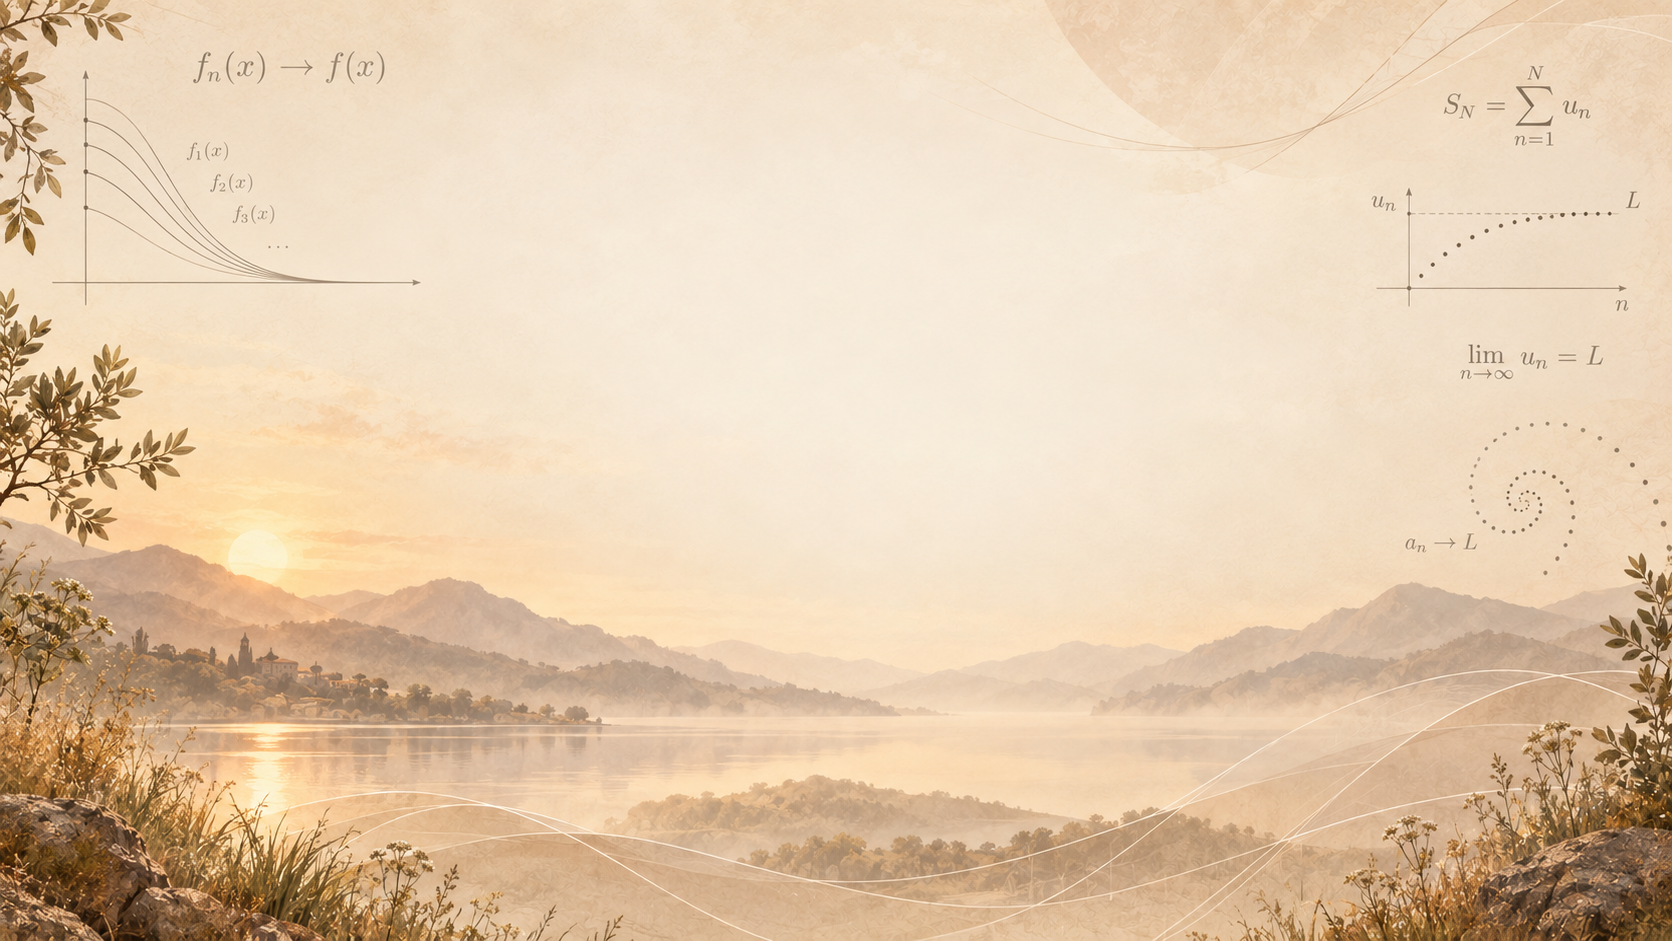
\includegraphics[width=\paperwidth,height=\paperheight,keepaspectratio=false]{chapter_07_bg_06.png}%
}
\section{The Weierstrass M-Test}

% --- Build 1/2 ---
\begin{frame}{Theorem 7.10: The Weierstrass M-Test}
  \begin{thmblock}{Theorem 7.10 (Weierstrass)}
    Suppose $\{f_n\}$ is a sequence of functions defined on $E$, and suppose
    \[
      |f_n(x)| \leq M_n \qquad (x \in E,\; n = 1, 2, 3, \dots).
    \]
    Then $\sum f_n$ \alert{converges uniformly} on $E$ if $\sum M_n$ converges.
  \end{thmblock}
  \hl{\small Here $M_n$ \emph{bounds the terms} $|f_n|$; it is not the error of Theorem 7.9.}

  \note{
    For series of functions, Weierstrass gave a very convenient test,
    Theorem 7.10. Suppose each "f" sub "n" is bounded on capital "E" by
    a constant capital "M" sub "n", the same for every "x". If the series
    of numbers capital "M" sub "n" converges, then the series of
    functions converges uniformly. As the line below the box notes,
    these capital "M" sub "n" bound the terms themselves; they are not
    the errors of Theorem 7.9. The test turns a question about functions
    into one about nonnegative numbers, where Chapter 3 gave us plenty
    of tools.
  }
\end{frame}

% --- Build 2/2 ---
\begin{frame}{Theorem 7.10: The Weierstrass M-Test}
  \begin{thmblock}{Theorem 7.10 (Weierstrass)}
    Suppose $\{f_n\}$ is a sequence of functions defined on $E$, and suppose
    \[
      |f_n(x)| \leq M_n \qquad (x \in E,\; n = 1, 2, 3, \dots).
    \]
    Then $\sum f_n$ \alert{converges uniformly} on $E$ if $\sum M_n$ converges.
  \end{thmblock}
  \hl{\small Here $M_n$ \emph{bounds the terms} $|f_n|$; it is not the error of Theorem 7.9.}
  \begin{remblock}{Remark}
    The \alert{converse} is \emph{not} asserted, and in fact it is not true.
  \end{remblock}

  \note{
    Rudin adds a remark in the gray box: the converse is not asserted,
    and in fact it is false. A series of functions can converge
    uniformly even though no choice of bounds capital "M" sub "n" has a
    convergent sum. We will see a simple example after the proof. So
    the M-test is a sufficient condition only. When it applies, it is
    extremely efficient; when it fails, we must look for another
    argument. Let's prove it.
  }
\end{frame}

% --- Build 1/2 ---
\begin{frame}{Proof of Theorem 7.10}
  \begin{proofblock}{Step 1: Tails of $\sum M_n$ are small}
    $\sum M_n$ converges, so by the Cauchy criterion for series (Theorem 3.22),
    for every $\varepsilon > 0$: \ $\sum_{i=n}^{m} M_i \leq \varepsilon$ \ for all
    $m \geq n$ large enough.
  \end{proofblock}

  \note{
    Let epsilon be given. The series of numbers, the sum of capital
    "M" sub "n", converges, so by the Cauchy criterion for series of
    numbers, Theorem 3.22, its blocks become small: there is a
    threshold such that for all "m" at least "n" beyond it, the sum of
    capital "M" sub "i" for "i" from "n" to "m" is at most epsilon.
    These are just numbers; there is no "x" anywhere yet. Next we
    transfer this to the functions.
  }
\end{frame}

% --- Build 2/2 ---
\begin{frame}{Proof of Theorem 7.10}
  \begin{proofblock}{Step 1: Tails of $\sum M_n$ are small}
    $\sum M_n$ converges, so by the Cauchy criterion for series (Theorem 3.22),
    for every $\varepsilon > 0$: \ $\sum_{i=n}^{m} M_i \leq \varepsilon$ \ for all
    $m \geq n$ large enough.
  \end{proofblock}
  \begin{proofblock}{Step 2: Transfer to $\sum f_n$ and apply Theorem 7.8}
    For the same $m, n$ and \alert{every} $x \in E$:
    \[
      |s_m(x) - s_{n-1}(x)| = \left|\sum_{i=n}^{m} f_i(x)\right|
      \leq \sum_{i=n}^{m} |f_i(x)| \leq \sum_{i=n}^{m} M_i \leq \varepsilon.
    \]
    So $\{s_n\}$ satisfies (13); by Theorem 7.8 it converges uniformly.
  \end{proofblock}

  \note{
    Now fix such "m" and "n", and take any "x" in capital "E". The
    difference of partial sums, "s" sub "m" of "x" minus the partial sum
    with index "n" minus 1, is the block of terms from "n" to "m". By the
    triangle inequality it is at most the sum of the absolute values,
    each bounded by capital "M" sub "i", so the block is at most
    epsilon, with a bound that does not depend on "x". That is condition
    13 for the partial sums, and Theorem 7.8 finishes the proof. We never
    needed to know the sum of the series.
  }
\end{frame}

% --- Build 1/2 ---
\begin{frame}{Example: A Trigonometric Series}
  \begin{exblock}{Applying the M-test}
    \[
      \sum_{n=1}^{\infty} \frac{\sin nx}{n^2}, \qquad
      \left|\frac{\sin nx}{n^2}\right| \leq \frac{1}{n^2} = M_n
      \quad (x \in \mathbb{R}), \qquad \sum \frac{1}{n^2} < \infty.
    \]
    $\Longrightarrow$ the series converges \alert{uniformly on all of $\mathbb{R}$}.
  \end{exblock}

  \note{
    Here is a typical application. Consider the series of sine of "n"
    "x" over "n" squared. Since the sine is bounded by 1, each term is
    at most 1 over "n" squared in absolute value, for every real "x".
    So we may take capital "M" sub "n" equal to 1 over "n" squared, and
    the series of 1 over "n" squared converges, as we know from
    Chapter 3. The M-test immediately gives uniform convergence on the
    whole real line, even though there is no elementary formula for
    the sum. Let's also estimate how fast it converges.
  }
\end{frame}

% --- Build 2/2 ---
\begin{frame}{Example: A Trigonometric Series}
  \begin{exblock}{Applying the M-test}
    \[
      \sum_{n=1}^{\infty} \frac{\sin nx}{n^2}, \qquad
      \left|\frac{\sin nx}{n^2}\right| \leq \frac{1}{n^2} = M_n
      \quad (x \in \mathbb{R}), \qquad \sum \frac{1}{n^2} < \infty.
    \]
    $\Longrightarrow$ the series converges \alert{uniformly on all of $\mathbb{R}$}.
  \end{exblock}

  \vspace{0.3em}
  \begin{hlbox}
  \textbf{Error bound, uniform in $x$:}
  \[
    |f(x) - s_N(x)| \leq \sum_{n > N} \frac{1}{n^2}
    < \sum_{n > N} \frac{1}{n(n-1)} = \boxed{\frac{1}{N}}
    \qquad (x \in \mathbb{R}).
  \]
  \end{hlbox}

  \note{
    The line below the box shows that the M-test also gives an explicit
    error bound. If "f" is the sum and "s" sub capital "N" the partial
    sum of the first capital "N" terms, the error at any point is the
    tail of the series, which is at most the tail of 1 over "n" squared.
    Each 1 over "n" squared is below 1 over the product "n" times "n"
    minus 1, and those fractions telescope to 1 over capital "N". So
    "s" sub capital "N" is within 1 over capital "N" of the sum at every
    point at once. Here is what that looks like.
  }
\end{frame}

\begin{frame}[c]{Example: Partial Sums of $\sum \frac{\sin nx}{n^2}$}
  \begin{center}
  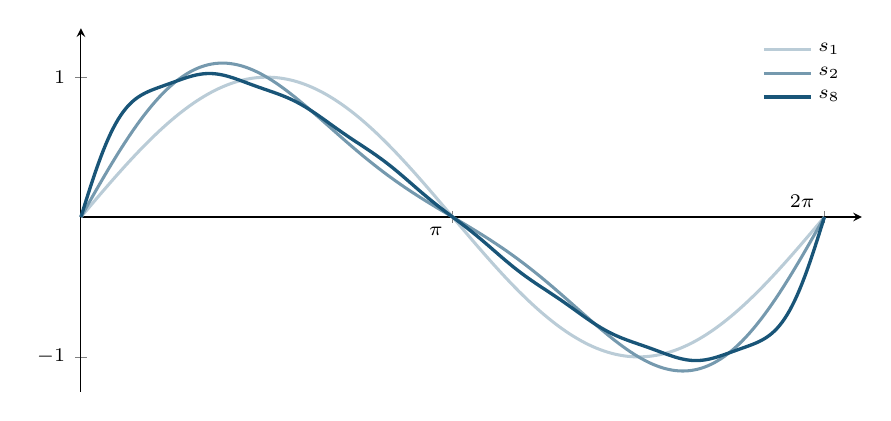
\begin{tikzpicture}
    \begin{axis}[
      width=11.5cm, height=6.2cm,
      axis lines=middle,
      xmin=0, xmax=6.6, ymin=-1.25, ymax=1.35,
      xtick={3.14159,6.28318}, xticklabels={},
      ytick={-1,1},
      tick label style={font=\scriptsize},
      legend style={font=\scriptsize, at={(0.99,0.99)}, anchor=north east,
        draw=none, fill=white, fill opacity=0.8, text opacity=1},
      clip=false,
    ]
      \addplot[defcolor!30, line width=1.1pt, domain=0:6.2832, samples=200]
        {sin(deg(x))};
      \addlegendentry{$s_1$}
      \addplot[defcolor!60, line width=1.1pt, domain=0:6.2832, samples=200]
        {sin(deg(x)) + sin(deg(2*x))/4};
      \addlegendentry{$s_2$}
      \addplot[defcolor, line width=1.2pt, domain=0:6.2832, samples=300]
        {sin(deg(x)) + sin(deg(2*x))/4 + sin(deg(3*x))/9 + sin(deg(4*x))/16
         + sin(deg(5*x))/25 + sin(deg(6*x))/36 + sin(deg(7*x))/49 + sin(deg(8*x))/64};
      \addlegendentry{$s_8$}
      \node[font=\scriptsize, anchor=north east] at (axis cs:3.14159,0) {$\pi$};
      \node[font=\scriptsize, anchor=south east] at (axis cs:6.28318,0) {$2\pi$};
    \end{axis}
  \end{tikzpicture}
  \end{center}

  \note{
    The picture shows partial sums over one period, from 0 to 2 pi. The
    light blue curve is "s" sub 1, just the sine of "x". The medium blue
    curve is "s" sub 2, which adds a quarter of the sine of 2 "x" and
    shifts the hump toward the left. The dark blue curve is "s" sub 8.
    All of them pass through 0 at "x" equals 0, pi, and 2 pi, since every
    term vanishes there. By the error bound, adding any further terms
    changes the dark curve by less than 1 over 8 anywhere, so it is
    already close to the sum. Notice that the corrections are small
    everywhere at once: there is no bad point where the partial sums lag
    behind, unlike the powers of "x" near 1. That is uniform convergence
    in action. Finally, why the converse of the M-test fails.
  }
\end{frame}

\begin{frame}{The Converse of the M-Test Fails}
  \begin{exblock}{Uniform convergence without a summable bound}
    Let $f_n(x) = \dfrac{(-1)^{n+1}}{n}$ (constant functions) on any set $E$.
    \begin{itemize}
      \item $\sum f_n$ converges \alert{uniformly}: the partial sums do not depend on $x$,
        and $\sum \frac{(-1)^{n+1}}{n}$ converges (Theorem 3.43)
      \item Any admissible bound has $M_n \geq |f_n(x)| = \frac{1}{n}$, so
        $\sum M_n = \alert{\infty}$
    \end{itemize}
  \end{exblock}

  \vspace{0.3em}
  \begin{hlbox}
  \textbf{Moral:} M-test is \emph{sufficient}, not necessary. Cancellation
  can give uniform convergence.
  \end{hlbox}

  \note{
    Here is a simple example showing that the converse of the M-test is
    false. Let each "f" sub "n" be a constant function: plus 1, then
    minus one half, then plus one third, and so on, with alternating
    signs. The partial sums are the partial sums of the alternating
    harmonic series, which converges by Theorem 3.43. Since nothing
    depends on "x", the convergence is automatically uniform. But any
    admissible bound capital "M" sub "n" must be at least 1 over "n", and
    the harmonic series diverges, so no choice of bounds has a finite
    sum. The moral: the M-test only sees the sizes of the terms, and
    whenever it applies, the series of absolute values converges too.
    Series that converge thanks to cancellation can be uniformly
    convergent while escaping the test. Let's summarize.
  }
\end{frame}
}

{
\usebackgroundtemplate{%
  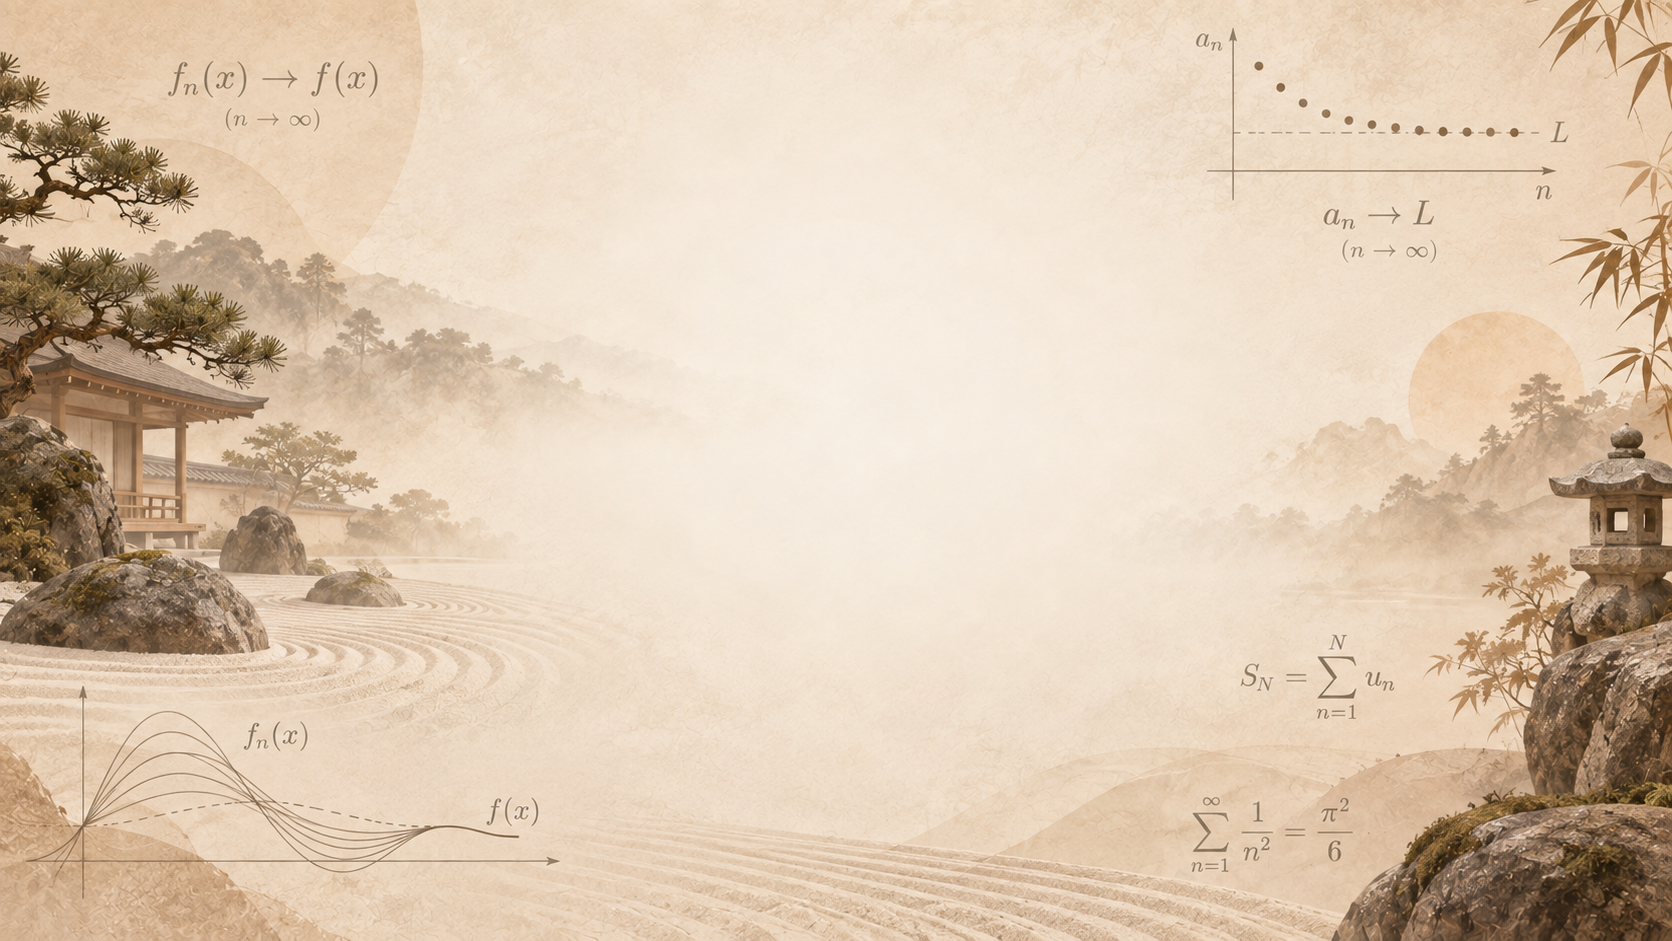
\includegraphics[width=\paperwidth,height=\paperheight,keepaspectratio=false]{chapter_07_bg_07.png}%
}
\section{Summary}

% --- Build 1/4 ---
\begin{frame}{Summary}
  \begin{hlbox}
  \textbf{Key takeaways from this section:}
  \begin{itemize}
    \item \textbf{Definition 7.7:} $f_n \to f$ \alert{uniformly} on $E$: one
      $N = N(\varepsilon)$ for all $x$;\\
      $f_n$ stays in the $\varepsilon$-tube
  \end{itemize}
  \end{hlbox}

  \note{
    Let's review. Definition 7.7 introduced uniform convergence: for
    every epsilon there is a single threshold capital "N", independent
    of the point, beyond which every "f" sub "n" is within epsilon of
    "f" on all of capital "E". Geometrically, the graph of "f" sub "n"
    lies entirely inside the epsilon tube around "f". Uniform
    convergence implies pointwise convergence, but not conversely, as
    the powers of "x" on the unit interval showed. Next, the Cauchy
    criterion.
  }
\end{frame}

% --- Build 2/4 ---
\begin{frame}{Summary}
  \begin{hlbox}
  \textbf{Key takeaways from this section:}
  \begin{itemize}
    \item \textbf{Definition 7.7:} $f_n \to f$ \alert{uniformly} on $E$: one
      $N = N(\varepsilon)$ for all $x$;\\
      $f_n$ stays in the $\varepsilon$-tube
    \item \textbf{Theorem 7.8 (Cauchy):} uniform $\iff$
      $|f_n - f_m| \leq \varepsilon$ on $E$ for $m, n \geq N$; \alert{no $f$ needed}
  \end{itemize}
  \end{hlbox}

  \note{
    Theorem 7.8, the Cauchy criterion, says that uniform convergence is
    equivalent to the functions "f" sub "n" and "f" sub "m" being
    uniformly close to each other for large indices. Its great virtue
    is that it does not mention the limit function. The proof used
    Theorem 3.11 to produce the pointwise limit and then let "m" go to
    infinity to get a bound uniform in "x". Next, the supremum
    criterion.
  }
\end{frame}

% --- Build 3/4 ---
\begin{frame}{Summary}
  \begin{hlbox}
  \textbf{Key takeaways from this section:}
  \begin{itemize}
    \item \textbf{Definition 7.7:} $f_n \to f$ \alert{uniformly} on $E$: one
      $N = N(\varepsilon)$ for all $x$;\\
      $f_n$ stays in the $\varepsilon$-tube
    \item \textbf{Theorem 7.8 (Cauchy):} uniform $\iff$
      $|f_n - f_m| \leq \varepsilon$ on $E$ for $m, n \geq N$; \alert{no $f$ needed}
    \item \textbf{Theorem 7.9:} uniform $\iff M_n = \sup_E |f_n - f| \to 0$;
      Examples 7.3, 7.6 fail, Example 7.5 passes
  \end{itemize}
  \end{hlbox}

  \note{
    Theorem 7.9 reduced uniform convergence to the worst case errors
    capital "M" sub "n", the supremum of the distance between "f" sub
    "n" and "f", tending to zero. With it we saw that Examples 7.3 and
    7.6 were not uniformly convergent, while Example 7.5 was, which
    warned us that uniform convergence alone does not control
    derivatives. Finally, the M-test.
  }
\end{frame}

% --- Build 4/4 ---
\begin{frame}{Summary}
  \begin{hlbox}
  \textbf{Key takeaways from this section:}
  \begin{itemize}
    \item \textbf{Definition 7.7:} $f_n \to f$ \alert{uniformly} on $E$: one
      $N = N(\varepsilon)$ for all $x$;\\
      $f_n$ stays in the $\varepsilon$-tube
    \item \textbf{Theorem 7.8 (Cauchy):} uniform $\iff$
      $|f_n - f_m| \leq \varepsilon$ on $E$ for $m, n \geq N$; \alert{no $f$ needed}
    \item \textbf{Theorem 7.9:} uniform $\iff M_n = \sup_E |f_n - f| \to 0$;
      Examples 7.3, 7.6 fail, Example 7.5 passes
    \item \textbf{Theorem 7.10 (M-test):} $|f_n| \leq M_n$, $\sum M_n < \infty$
      $\Rightarrow$ $\sum f_n$ uniform; converse false
  \end{itemize}

  \vspace{0.2em}
  \textbf{Next:} uniform limits of continuous functions are \alert{continuous}.
  \end{hlbox}

  \note{
    Theorem 7.10, the Weierstrass M-test, says that if each term of a
    series of functions is bounded by a constant capital "M" sub "n",
    and the sum of the constants converges, then the series converges
    uniformly. It is sufficient but not necessary. In the next
    section, Uniform Convergence and Continuity, we reap the first
    reward: we will prove that a uniform limit of continuous functions
    is continuous, so the two limit processes from the main problem
    can be interchanged. This is exactly what failed in Example 7.3.
    See you next time.
  }
\end{frame}
}

\end{document}
